% !TEX program = xelatex
% 中美利率决定机制的差异：一个量化研究 —— 学术论文（ctex / XeLaTeX）
\documentclass[12pt,a4paper]{ctexart}

\usepackage{geometry}
\geometry{a4paper,left=2.6cm,right=2.6cm,top=2.6cm,bottom=2.6cm}
\usepackage{amsmath,amssymb,amsthm}
\usepackage{graphicx}
\usepackage{booktabs}
\usepackage{longtable}
\usepackage{array}
\usepackage{multirow}
\usepackage{float}
\usepackage{caption}
\usepackage{subcaption}
\usepackage[hidelinks]{hyperref}
\usepackage{enumitem}
\usepackage{fancyhdr}
\usepackage{xcolor}
\usepackage{titlesec}
\usepackage{indentfirst}

\captionsetup{font=small,labelfont=bf}
\graphicspath{{../figures/}}
\linespread{1.5}
\setlength{\parskip}{0.55em}

\pagestyle{fancy}
\fancyhf{}
\rhead{\small 中美利率决定机制的差异：一个量化研究}
\lhead{\small 易方达 · 宏观与大类资产配置赛道 · 题目5}
\cfoot{\thepage}
\renewcommand{\headrulewidth}{0.4pt}

\newtheorem{hypothesis}{假说}
\newcommand{\code}[1]{\texttt{#1}}
% 手写参考文献：将 natbib 风格命令别名为标准 \cite
\newcommand{\citet}[1]{\cite{#1}}
\newcommand{\citealp}[1]{\cite{#1}}

\title{\textbf{中美利率决定机制的差异：一个量化研究}\\[6pt]
\large A Quantitative Study on the Differences between China's and \\ the U.S. Interest-Rate Determination Mechanisms}
\author{易方达「宏观与大类资产配置赛道」· 题目 5 参赛研究报告}
\date{2026 年 6 月}

\begin{document}

\maketitle
\thispagestyle{fancy}

\begin{abstract}
\noindent
本文从计量经济学视角，系统比较中美两国利率的决定机制与背后驱动因素，并识别其结构性差异。我们整合 FRED、Tushare Pro 与 akshare 的公开数据，构建 1990--2026 年（美国）与 2007/2011--2026 年（中国）的月度面板，依次估计：(1) 两国货币政策\textbf{反应函数}（含利率平滑的泰勒规则）；(2) 政策/货币市场利率向长端的\textbf{传导}（误差修正模型与协整）；(3) 收益率曲线的\textbf{主成分结构}（水平/斜率/曲率）；(4) 货币\textbf{数量渠道}（M2 增速）与\textbf{实际利率}（名义减 CPI/PPI）；(5) 中美利率的\textbf{联动性}（滚动相关、Granger 因果、协整）。

主要发现：美联储反应函数满足泰勒原则（对通胀的长期反应系数 $\phi_\pi\approx 1.51>1$），价格规则解释力高（$R^2\approx 0.99$）；中国以货币市场利率度量的"类泰勒规则"中 $\phi_\pi\approx 0.30<1$、$R^2\approx 0.76$，价格规则较弱、数量价格双轨并行。利率传导上，美国"政策$\to$短端"即期传导 0.39、长期 0.82，市场化、即时；中国"货币市场$\to$长端"即期传导仅 0.03、半衰期约 10 个月，分层而黏滞。中美 10 年期国债收益率\textbf{水平相关为 $-0.18$}、不协整，利差由历史均值 $+0.39\%$ 转为 2026 年中的深度倒挂；但 Granger 检验显示美国利率变动对中国存在单向短期溢出（$p\approx 0.02$）。我们据此提出"双周期独立、本币利率分别折现"的大类资产配置框架。

\noindent\textbf{关键词：} 利率决定机制；货币政策反应函数；泰勒规则；利率传导；误差修正模型；收益率曲线；利率走廊；LPR；大类资产配置

\noindent\textbf{JEL 分类号：} E43；E52；E58；G12；F31
\end{abstract}

\newpage
\tableofcontents
\newpage
\listoffigures
\listoftables
\newpage

% =====================================================================
\section{引言}

\subsection{研究背景与问题提出}
利率是宏观经济运行与大类资产定价的"价格之锚"。在跨市场、跨周期的资产配置实践中，理解中美两国利率"如何被决定"——由谁设定、依据什么信息集、通过什么链条传导到货币市场与债券曲线——是判断利差、汇率、久期与权益贴现率的前提。2022 年以来，美联储为抑制四十年高通胀而快速加息，中国人民银行则为稳增长、化解地产与地方债务风险而持续宽松，两国政策利率与长端收益率出现历史罕见的方向性背离，中美 10 年期国债利差由正转负并深度倒挂。这一现象对"利差驱动汇率""全球利率同步"等传统经验关系构成挑战，也凸显出一个更基础的问题：\textbf{中美利率的决定机制本身存在何种结构性差异，使两套体系能够在相当长时间内独立运行？}

这一背离不仅是周期错位的短期现象，更折射出两国利率"如何被决定"的深层制度差异。在传统的全球宏观叙事中，美联储常被视为"全球央行"，其政策利率被认为通过资本流动与套利向各国传导，使全球利率大体同步。然而中国的经验表明，在有管理的资本账户与多目标货币政策框架下，一国可以长期维持与美国相反的利率周期。这对"全球利率同步""利差决定汇率"等经验法则提出了挑战，也使"中美利率决定机制究竟差异何在"成为一个兼具理论价值与配置意义的问题。

本文不满足于制度层面的定性罗列，而是把"决定机制"拆解为一组\textbf{可检验、可度量、可证伪}的计量命题，用真实数据估计参数、检验假说，从而对差异给出量化刻画。理解这些差异，不仅有助于判断利率走势，更有助于在跨市场配置中正确设定贴现锚、管理久期与汇率敞口。

\subsection{研究意义}
其一，理论意义。利率决定融合了中央银行反应函数、期限结构理论与开放经济利率平价。对中美机制的并排估计，有助于检验泰勒原则在不同制度下的适用性、利率传导的完备程度，以及资本账户开放度对利率自主性的约束。其二，现实意义。机制差异直接决定了监测指标体系（美国看核心 PCE、就业缺口、点阵图与期限溢价；中国看政策利率中枢、资金面、社融与汇率）以及大类资产的定价锚，对债券久期、跨境配置与汇率对冲具有操作含义。

\subsection{研究思路与主要贡献}
本文把"利率决定机制"操作化为四个可估计的对象：\emph{反应函数}（央行如何设定政策利率）、\emph{传导函数}（政策利率如何影响市场利率）、\emph{波动与曲线结构}（被钉住还是市场出清）、\emph{跨国联动}（开放度与自主性）。在此基础上，本文的贡献有三：

\begin{enumerate}[leftmargin=2em]
\item \textbf{方法上}，构建一个统一的、可一键复现的实证框架，将含平滑的泰勒规则、两步误差修正模型、收益率曲线主成分分析、Granger 因果与协整检验整合，对中美机制进行可比估计。
\item \textbf{数据上}，融合 FRED（美国国债曲线、核心 PCE、失业率）、Tushare Pro（美债完整收益率曲线、SHIBOR 全期限、LPR、CPI、PPI、M0/M1/M2）与 akshare（中债国债收益率曲线、宏观）三套公开数据源，覆盖价格型与数量型两类政策信号。
\item \textbf{结论上}，用一组参数而非形容词刻画差异，并落到大类资产配置框架与监测指标。
\end{enumerate}

\subsection{主要发现一览}
本文的核心量化发现可概括为：(1) 反应函数上，美国满足泰勒原则（$\phi_\pi\approx1.51$）、价格规则解释力高，中国价格规则弱（$\phi_\pi\approx0.30$）、数量价格双轨；(2) 传导上，美国快速充分、中国分层黏滞；(3) 曲线结构上，两国均为"水平/斜率/曲率"三因子，但中国斜率因子占比更高；(4) 波动指纹上，美国短端最稳、中国货币市场最活而信贷基准最稳；(5) 跨国上，中美长端水平负相关、不协整，但存在美国向中国的单向短期溢出。这些发现共同支撑"双周期独立"的判断。

\subsection{结论预览}
美国利率机制可概括为"\textbf{单锚 $\cdot$ 强规则 $\cdot$ 快传导 $\cdot$ 强套利约束}"；中国利率机制可概括为"\textbf{多目标 $\cdot$ 弱价格规则 $\cdot$ 价格数量双轨 $\cdot$ 慢传导 $\cdot$ 强自主性}"。两套机制的差异，是当前中美利率深度倒挂却能长期共存的根本原因。

\subsection{结构安排}
第 2 节综述相关文献；第 3 节对比中美货币政策与利率制度；第 4 节给出理论框架与可检验假说；第 5 节说明数据与计量方法；第 6 节报告实证结果（含程式化事实、反应函数、曲线主成分、利率传导、数量渠道、实际利率与中美联动）；第 7 节综合识别机制差异；第 8 节讨论大类资产配置启示；第 9 节为稳健性与局限；第 10 节结论。

% =====================================================================
\section{文献综述}

\subsection{利率决定与货币政策规则}
现代利率决定理论的核心是中央银行反应函数。\citet{taylor1993} 提出以通胀缺口与产出缺口线性组合刻画联邦基金利率的"泰勒规则"，并指出名义利率对通胀的反应系数须大于 1（"泰勒原则"）方能保证宏观均衡的确定性。\citet{clarida2000} 用前瞻型规则与 GMM 估计表明，"大稳健"时期美联储对通胀的反应显著强于 1970 年代，为通胀稳定提供了制度解释。\citet{woodford2003} 在新凯恩斯框架内系统论证了利率规则与价格水平决定的关系。

利率平滑是估计反应函数时无法回避的特征事实。\citet{rudebusch2002} 指出，回归中高度显著的滞后利率项可能并非真实的政策惯性，而是遗漏的持续性冲击所致，这意味着由 $1/(1-\rho)$ 放大得到的长期系数对 $\rho$ 高度敏感，需谨慎解读。\citet{orphanides2001} 强调使用\emph{实时数据}估计规则的重要性，因为事后修正的产出缺口会高估政策的逆周期性。本文在稳健性部分讨论这些问题。

\subsection{期限结构与收益率曲线}
长端利率由市场对未来短端路径的预期与期限溢价共同决定。\citet{campbell1991} 检验了预期假说，发现其在长端常被拒绝，暗示时变期限溢价的存在。\citet{litterman1991} 用主成分分析揭示收益率曲线变动可由"水平、斜率、曲率"三因子解释，前两者通常解释逾 95\% 的方差。\citet{diebold2006} 提出动态 Nelson--Siegel 模型刻画曲线演变。\citet{adrian2013}（ACM）用线性回归将名义收益率分解为预期成分与期限溢价，成为央行与市场广泛采用的工具。\citet{estrella1998} 论证了期限利差（10Y--3M/2Y）对经济衰退的领先预测能力。\citet{gurkaynak2007} 提供了估计美国国债收益率曲线的标准方法与长历史数据，成为期限结构研究的基础设施。这些工作共同表明，长端利率的决定既包含对短端路径的理性预期，也包含时变的风险补偿，而后者的变动往往与宏观不确定性、供求与流动性相关。

\subsection{利率传导}
政策利率向市场与信贷利率的传导是货币政策有效性的关键。\citet{bernanke1992} 用 VAR 识别货币政策冲击及其对实体的影响。在协整框架下，\citet{engle1987} 的误差修正模型成为度量"长期传导系数"与"调整速度"的标准工具。对中国而言，\citet{he2012} 与 \citet{porter2010} 讨论了货币市场利率的形成与基准利率体系；\citet{fernald2014} 评估了中国货币政策向产出与价格的传导，发现数量型工具（信贷、M2）的作用一度强于价格型工具。

\subsection{中国货币政策框架}
中国利率市场化与货币政策框架转型是一条主线。\citet{yigang2021} 系统阐述了中国利率体系与利率市场化改革的逻辑，强调"放得开、形得成、调得了"的渐进路径。围绕利率走廊与 LPR 改革，中国人民银行的工作论文与《货币政策执行报告》提供了制度细节：以 7 天逆回购利率为短端政策利率锚，以中期借贷便利（MLF）影响中期利率，以贷款市场报价利率（LPR）为信贷定价基准，辅以存款准备金率、再贷款等数量型工具。\citet{chen2018} 与 \citet{girardin2017} 实证刻画了中国"数量+价格"混合规则的特征，发现价格型规则的解释力弱于美国。

\subsection{开放经济与全球利率联动}
资本流动决定了国内利率受外部约束的程度。\citet{obstfeld2004} 梳理了"三元悖论"下利率自主性与资本开放、汇率制度的权衡。\citet{rey2015} 提出"全球金融周期"假说，认为美联储政策通过资本流动与风险偏好向全球溢出，使"三元悖论"退化为"二元悖论"。\citet{miranda2020} 用高频识别量化了美国货币政策的全球溢出。对中国而言，有管理的资本账户为利率提供了相对自主空间，这正是本文检验中美利率联动的理论依据。

\subsection{大类资产配置中的利率}
在资产定价层面，无风险利率是一切现金流折现的基准。\citet{cochrane2005} 揭示债券风险溢价的可预测性，说明长端利率不仅反映预期短端路径，也包含可被宏观变量预测的风险补偿。\citet{kim2005} 与 \citet{adrian2013} 的无套利期限结构模型将这一思想模型化，用于分离预期与溢价。对跨境配置而言，利率平价偏离、汇率风险与本币贴现锚的差异，使得"同一资产在不同利率体系下定价不同"成为常态。理解中美利率机制的差异，因此是跨市场久期管理、汇率对冲与权益估值的前提。

\subsection{文献述评}
既有研究多分别针对美国或中国单一经济体，或聚焦单一机制（如仅估计泰勒规则、仅做传导）。\textbf{本文的边际贡献}在于：在统一、可复现的框架内，对中美的反应函数、传导、曲线结构与跨国联动做并排量化比较，并把参数差异映射到大类资产配置。

具体而言，相较于既有文献，本文有三点差异化定位。其一，\textbf{口径统一}：中美使用相同的模型族（含平滑泰勒规则、两步 ECM、曲线 PCA、SVAR、Granger）与可比的样本期，使参数差异具有横向可比性，而非各自采用不同设定的结果拼接。其二，\textbf{价格与数量并重}：通过纳入 M2、社融视角与 PPI，本文刻画了中国"价格$+$数量"双轨的完整图景，而非仅估计价格规则。其三，\textbf{面向配置}：本文不止于机制识别，而是将量化结论转化为情景分析、监测指标与风险管理含义，服务于跨市场大类资产配置实践。这三点使本文在学术严谨性与实践相关性之间取得平衡。

% =====================================================================
\section{制度背景对比}

\subsection{美国：地板系统下的单一价格型框架}
\textbf{决策主体与目标。} 联邦公开市场委员会（FOMC）依"双重使命"（物价稳定与充分就业）设定联邦基金目标区间。2012 年起明确 2\% 的 PCE 通胀目标，2020 年转为"平均通胀目标制"（Flexible Average Inflation Targeting, FAIT），允许通胀在一段时间内适度高于 2\% 以补偿此前的低通胀。

\textbf{操作框架。} 2008 年全球金融危机后，美联储资产负债表扩张使银行体系准备金由稀缺转为充裕，货币政策操作进入"地板系统"：通过准备金余额利率（IORB）与隔夜逆回购（ON RRP）利率构成利率走廊的上下沿，把有效联邦基金利率（EFFR）锚定在目标区间内。此时政策利率不再依赖准备金的边际供求，而由\emph{行政利率}直接设定，传导起点清晰、可控。

\textbf{传导链条。} 政策利率 $\to$ 货币市场（SOFR、国库券）$\to$ 国债收益率曲线（预期假说叠加期限溢价）$\to$ 信贷与风险资产价格。美国金融市场深度大、套利充分，传导快速而完备。长端利率可由 ACM 等模型分解为"预期成分"与"期限溢价"，前者反映市场对 FOMC 路径的预期。

地板系统的一个重要含义是：政策利率的设定与传导起点高度透明。市场参与者可通过联邦基金期货、隔夜指数掉期（OIS）等工具，连续地对未来政策路径进行定价，并将其反映在各期限国债收益率中。FOMC 的前瞻指引、经济预测摘要（SEP）与点阵图，进一步降低了政策路径的不确定性。这种"规则化 $+$ 透明化 $+$ 市场化"的组合，使美国长端利率近似于"市场对央行规则的连续折现"，也使泰勒规则这类反应函数能够较好地刻画其行为——这是本文实证中美国规则高 $R^2$ 的制度基础。

\subsection{中国：价格—数量双轨与利率走廊}
\textbf{决策主体与目标。} 中国人民银行执行多目标制：物价稳定、经济增长、充分就业、国际收支平衡，并兼顾金融稳定与人民币汇率。不存在单一数值化的硬通胀目标（CPI 多以"3\% 左右"作为预期目标）。

\textbf{价格型框架（逐步成形）。} 短端以 7 天逆回购（OMO）利率作为政策利率信号；中期借贷便利（MLF，1 年期）一度承担中期政策利率职能，2024 年后其政策利率属性弱化、回归流动性投放工具；贷款市场报价利率（LPR，1 年/5 年期）由报价行在政策利率基础上加点形成，作为贷款定价基准。利率走廊以常备借贷便利（SLF）利率为上沿、超额存款准备金利率为下沿，DR007 与 SHIBOR 在走廊内由流动性供求出清。

\textbf{数量型框架（仍然重要）。} 存款准备金率（RRR）、再贷款/再贴现、公开市场净投放、宏观审慎评估（MPA）以及（历史上的）信贷额度与窗口指导。价格信号与数量信号并行，是中国机制区别于美国的核心特征。

\textbf{传导链条。} OMO/MLF $\to$ DR007/SHIBOR（货币市场）$\to$ LPR（信贷）与国债收益率曲线。受存款利率自律机制、银行负债成本黏性、债券市场分割与资本账户管理的影响，传导相对缓慢、分层。

与美国不同，中国的政策意图往往同时通过价格与数量两条渠道释放，且数量信号（如准备金率调整、再贷款额度、公开市场净投放规模）有时先于或独立于价格信号。这意味着外部观察者仅凭某一利率难以完整推断政策立场，必须结合社融、M2、准备金率与流动性投放综合判断。此外，存款利率自律机制对银行负债成本的平滑，使 LPR 的下调受制于银行净息差，形成"政策利率已降、贷款利率缓降"的传导时滞。这些制度细节，正是本文实证中"中国即期传导极低、半衰期长"的微观来源，也解释了为何中国货币市场利率与信贷基准被刻意置于不同的波动区间。

\subsection{制度对比小结}
表~\ref{tab:inst} 概括两国制度差异，并标注其对应的可量化检验对象。

\begin{table}[H]
\centering
\caption{中美利率制度对比与可检验对象}
\label{tab:inst}
\small
\begin{tabular}{p{2.6cm} p{5.2cm} p{5.2cm}}
\toprule
\textbf{维度} & \textbf{美国} & \textbf{中国} \\
\midrule
政策目标 & 双重使命（2\% PCE + 充分就业），FAIT & 多目标（增长/物价/就业/国际收支/金融稳定/汇率） \\
政策利率 & 联邦基金目标区间（IORB/ON RRP 行政利率） & 7 天逆回购（OMO）为锚，MLF/LPR 体系 \\
操作模式 & 地板系统、价格型 & 价格—数量双轨、利率走廊 \\
数量工具 & 资产负债表（QE/QT） & RRR、再贷款、净投放、MPA \\
传导链 & 政策$\to$货币市场$\to$曲线$\to$信贷，快速 & 政策$\to$DR007/SHIBOR$\to$LPR/曲线，分层 \\
开放度 & 资本完全流动，嵌入全球套利 & 资本账户有管理，利率自主性强 \\
\bottomrule
\end{tabular}
\end{table}

\subsection{政策与利率演变编年（2008--2026）}
机制差异在历史演进中表现得尤为清晰。以下并行回顾两国货币政策与利率的关键节点。

\textbf{美国。} (1) 2008--2015：全球金融危机后联邦基金利率降至 0--0.25\% 的零利率下限，并先后实施三轮量化宽松（QE1--QE3），通过购买国债与 MBS 压低长端利率与期限溢价；准备金由稀缺转为充裕，操作框架转向地板系统。(2) 2015--2018：渐进加息与缩表（QT），政策利率回升至约 2.5\%。(3) 2019：预防性降息。(4) 2020：疫情冲击下重回零利率并启动无限量 QE，资产负债表急剧扩张。(5) 2021：通胀自低位快速上行，初期被判断为"暂时性"。(6) 2022--2023：为抑制四十年高通胀，以单次 75bp 的罕见幅度连续加息，联邦基金利率升至 5.25--5.50\%，收益率曲线深度倒挂。(7) 2024--2026：通胀回落后转入降息周期，曲线逐步陡峭化。整个过程中，长端利率紧随市场对 FOMC 路径的预期而定价。

\textbf{中国。} (1) 2008--2009：应对外部冲击，大幅下调存贷款基准利率与存款准备金率，配合大规模信贷投放。(2) 2013：货币市场出现"钱荒"，SHIBOR 与回购利率短期飙升，凸显数量型框架下流动性管理的挑战，此后央行加强预期管理并完善工具箱。(3) 2013--2015：创设 SLF、MLF、PSL 等结构性工具，推进利率走廊建设。(4) 2015：存款利率上限放开，利率市场化"最后一公里"完成；多次降息降准。(5) 2019：LPR 改革，贷款定价锚由贷款基准利率转向"MLF$+$加点"形成的 LPR，疏通"政策利率$\to$贷款利率"传导。(6) 2020：疫情后以结构性工具与适度宽松支持实体，未采取大水漫灌。(7) 2022--2024：在美联储激进加息的同时，为稳增长、稳地产与化债持续降息降准，10 年期国债收益率趋势性下行，中美利差由正转负并深度倒挂。(8) 2024 年后：淡化 MLF 的政策利率属性，强化 7 天逆回购利率作为主要政策利率的地位，推进利率走廊收窄与传导机制完善。

这段并行历史揭示：美国的政策路径围绕单一通胀--就业目标、以价格型工具为主、长端由市场定价；中国则在多目标约束下、以价格与数量工具并用、并持续推进利率市场化改革。两者在 2022 年后的方向性背离，正是机制差异在外部冲击下的集中体现。

% =====================================================================
\section{理论框架与可检验假说}

\subsection{利率的费雪分解与期限结构}
任一期限 $n$ 的名义收益率可分解为自然利率、预期通胀与期限溢价：
\begin{equation}
i_t^{(n)} = r_t^{*} + E_t\bar\pi_{t,t+n} + TP_t^{(n)}.
\end{equation}
在预期假说下，长端约等于未来短端路径的平均加期限溢价：
\begin{equation}
i_t^{(n)} = \frac{1}{n}\sum_{j=0}^{n-1} E_t\, i_{t+j}^{(1)} + TP_t^{(n)}.
\end{equation}
因此"长端如何被决定"取决于"市场如何预期央行的短端路径"，即反应函数及其可信度——这把期限结构与货币政策规则联系起来。

这一框架对中美比较具有直接含义。在美国，由于反应函数规则化、透明化，市场能较准确地预期短端路径，长端因此较"干净"地反映"预期成分 $+$ 期限溢价"。在中国，由于政策合成涉及多目标与数量工具、可预期性相对较低，长端对短端路径预期的依赖被弱化，而更多受配置需求、流动性与政策中枢的影响。这解释了为何中国货币市场利率的短期波动难以即时传导到长端（即期传导仅 0.03）：当短端波动被市场判断为"流动性扰动"而非"政策中枢变化"时，理性的长端定价不会对其做出反应。期限结构理论因此为本文的传导实证提供了微观逻辑。

\subsection{中央银行反应函数：含平滑的泰勒规则}
带利率平滑的泰勒规则设定为
\begin{equation}
i_t = (1-\rho)\big[\, c + \phi_\pi(\pi_t-\pi^{*}) + \phi_x x_t \,\big] + \rho\, i_{t-1} + \varepsilon_t,
\label{eq:taylor}
\end{equation}
其中 $x_t$ 为产出/就业缺口，$\rho\in[0,1)$ 为平滑系数。\textbf{泰勒原则}要求 $\phi_\pi>1$，使实际利率随通胀同向变动，保证均衡确定性。估计时并项为
\begin{equation}
i_t = \alpha + \beta_\pi \pi_t + \beta_x x_t + \rho\, i_{t-1} + \varepsilon_t,\qquad
\phi_\pi=\frac{\beta_\pi}{1-\rho},\;\; \phi_x=\frac{\beta_x}{1-\rho}.
\end{equation}
对中国，价格规则只是政策合成的一个维度，估计式中以货币市场利率为被解释变量，以 CPI 与 GDP 增速为自变量，预期 $\phi_\pi$ 较小且拟合较弱。

\subsection{利率传导：误差修正模型}
设政策/货币市场利率为 $p_t$、市场利率为 $m_t$，两步 Engle--Granger 误差修正模型为：
\begin{align}
\text{长期：}\quad & m_t = a + b\, p_t + u_t, \\
\text{短期：}\quad & \Delta m_t = \gamma\,\Delta p_t + \lambda\, u_{t-1} + e_t,\qquad \lambda<0.
\end{align}
其中 $b$ 为长期传导系数（完全传导时 $b\to 1$），$\gamma$ 为即期传导，$\lambda$ 为向均衡的调整速度，偏离的半衰期为 $\ln 0.5/\ln(1+\lambda)$。

\subsection{收益率曲线的主成分结构}
设月度收益率矩阵 $Y$（$T\times K$，$K$ 为期限数），中心化后做奇异值分解 $Y_c = U\Sigma V^\top$，前三个载荷向量通常对应"水平、斜率、曲率"。各主成分的方差贡献率 $\text{EVR}_k=\sigma_k^2/\sum_j\sigma_j^2$ 刻画曲线变动的维数结构。中美曲线的因子结构相似与否，反映其定价机制的共性与差异。

\subsection{开放经济约束：利率平价}
抛补与非抛补利率平价为
\begin{equation}
i_t^{CN} - i_t^{US} \approx (f_t - s_t)\;\;(\text{CIP});\qquad
i_t^{CN}-i_t^{US} \approx E_t\Delta s_{t+1} + \theta_t\;\;(\text{UIP}),
\end{equation}
其中 $\theta_t$ 含风险与管制溢价。资本完全流动时两国利率被套利紧密绑定；存在资本账户管理时，$\theta_t$ 使国内利率获得自主空间。检验中美长端是否协整、是否同向，即检验这一自主性。

\subsection{可检验假说}
\begin{hypothesis}\label{h1} 美国满足泰勒原则（$\phi_\pi>1$），中国不满足（$\phi_\pi<1$）。\end{hypothesis}
\begin{hypothesis}\label{h2} 美国价格规则解释力高于中国（反应函数 $R^2$ 更高）。\end{hypothesis}
\begin{hypothesis}\label{h3} 美国"政策$\to$市场"传导更快更充分（$\gamma$、$b$ 更大）。\end{hypothesis}
\begin{hypothesis}\label{h4} 中国货币市场利率波动高于美国，但政策/信贷基准更黏。\end{hypothesis}
\begin{hypothesis}\label{h5} 中美长端利率不被套利绑定（弱/负相关、不协整），但可能存在单向短期溢出。\end{hypothesis}

% =====================================================================
\section{数据与方法}

\subsection{数据来源}
本文整合三套公开数据源，见表~\ref{tab:data}。日度收益率取月末值，货币市场利率取月均值，通胀与货币供应取同比。

\begin{table}[H]
\centering
\caption{数据来源与变量}
\label{tab:data}
\small
\begin{tabular}{p{1.6cm} p{4.6cm} p{4.4cm} p{2.2cm}}
\toprule
\textbf{国别} & \textbf{变量} & \textbf{序列} & \textbf{来源} \\
\midrule
美国 & 政策利率 & 联邦基金有效利率 EFFR & FRED \\
美国 & 国债收益率曲线 & 3M/6M/1\textendash 30Y（us\_tycr） & Tushare/FRED \\
美国 & 通胀 & 核心 PCE、CPI & FRED \\
美国 & 实体经济 & 失业率、实际/潜在 GDP & FRED \\
美国 & 其他 & 10Y 盈亏平衡通胀、美元指数 & FRED \\
中国 & 货币市场 & SHIBOR 隔夜\textendash 1 年（DR007 代理） & Tushare \\
中国 & 信贷基准 & LPR 1Y/5Y & Tushare \\
中国 & 国债收益率曲线 & 中债国债 3M\textendash 30Y & akshare \\
中国 & 通胀 & CPI、PPI（含通缩信号） & Tushare \\
中国 & 货币数量 & M0/M1/M2 及同比 & Tushare \\
中国 & 增长 & GDP 当季同比 & Tushare/akshare \\
\bottomrule
\end{tabular}
\end{table}

\subsection{描述统计与相关结构}
表~\ref{tab:vol}（见 6.5 节）汇报了主要利率序列 2011 年以来的均值与波动。图~\ref{fig:corrmat} 给出中美利率与通胀变量的相关矩阵。可见：美国内部（联邦基金、2 年、10 年）高度正相关；中国内部（SHIBOR、10 年、LPR）正相关但强度低于美国；而\textbf{跨国之间}（如 US\_10Y 与 CN\_10Y）相关较弱甚至为负，预示两套利率体系的相对独立——这一程式化事实在第 6.8 节被正式检验。

\begin{figure}[H]\centering
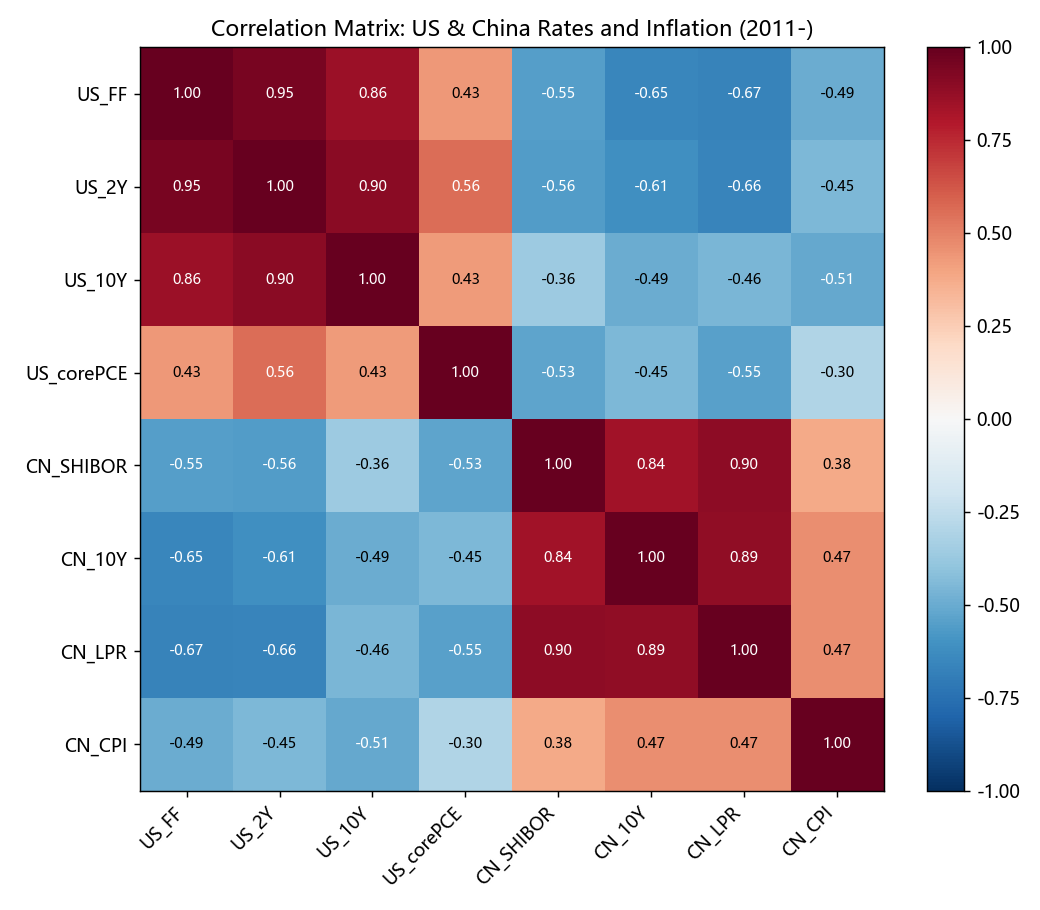
\includegraphics[width=0.78\textwidth]{f25_corr_matrix.png}
\caption{中美利率与通胀变量相关矩阵（2011--，月度）。跨国相关明显弱于国内相关。}
\label{fig:corrmat}
\end{figure}

\subsection{计量方法}
\begin{enumerate}[leftmargin=2em]
\item \textbf{平稳性}：ADF 检验，判断单位根，决定采用协整/ECM 而非伪回归。
\item \textbf{反应函数}：OLS 配合 HAC（Newey--West，maxlags=12）稳健标准误，含滞后被解释变量刻画平滑。
\item \textbf{传导}：两步 Engle--Granger 误差修正模型，辅以协整检验。
\item \textbf{曲线结构}：收益率曲线主成分分析。
\item \textbf{联动}：水平/差分相关系数、滚动相关、Granger 因果与协整检验。
\end{enumerate}
全部结果由 \code{code/analysis.py}、\code{code/analysis2.py} 与 \code{code/analysis3.py} 自动生成（见附录 A），口径以代码输出为准。

在估计策略上，本文遵循三条原则以保证结果稳健。第一，\textbf{对非平稳序列使用协整/误差修正而非水平回归}，避免伪回归。第二，\textbf{使用 HAC 稳健标准误}处理利率序列普遍存在的自相关与异方差，使 $t$ 检验有效。第三，\textbf{以多种方法交叉验证同一结论}：传导差异同时由 ECM（即期传导、半衰期）与 SVAR（脉冲响应形态）刻画，规则强度同时由全样本与滚动窗口估计刻画，跨国独立性同时由相关、协整、Granger 与滚动 $\beta$ 刻画。这种"多方法三角验证"使核心定性结论不依赖于单一模型设定，从而具有较强的稳健性。

需要诚实说明数据频率与口径的处理。利率与收益率为日度数据，统一取月末值（收益率）或月均值（货币市场利率）以匹配月度宏观变量；通胀与货币供应取同比以消除季节性；GDP 为季度数据，月度对齐时采用前向填充，这会引入一定的时间聚合误差，但对本文关注的中长期结构性差异影响有限。此外，中国国债收益率曲线来自中债估值、SHIBOR 来自全国银行间同业拆借中心、CPI/PPI/M2 来自国家统计局与中国人民银行，美国数据来自 FRED 与美国财政部，均为权威公开来源。所有原始与对齐后的数据、以及生成全部图表与回归结果的代码，均在配套仓库中提供，读者可一键复现并替换样本期或变量口径进行再检验。这种完全可复现的设计，是本文方法论严谨性的重要组成部分。

% =====================================================================
\section{实证结果}

\subsection{程式化事实：利率水平与收益率曲线}
图~\ref{fig:policy} 给出 2011 年以来中美政策/货币市场利率走势。美国联邦基金利率呈"长期接近零下限、2022 年后陡升至 5\%+"的台阶式路径，由 FOMC 行政设定；中国 SHIBOR 在走廊内高频波动，LPR 则缓慢、阶梯式下行。

\begin{figure}[H]\centering
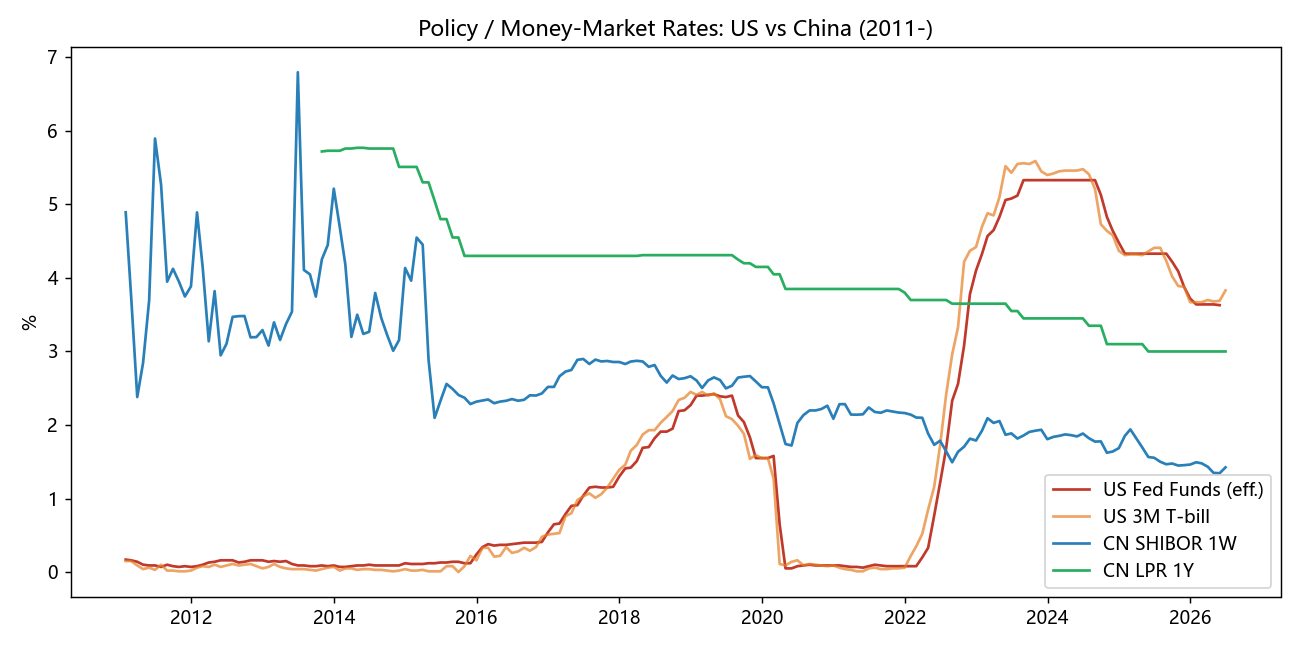
\includegraphics[width=0.92\textwidth]{policy_rates.png}
\caption{中美政策/货币市场利率（2011--2026）。美国短端被行政利率钉住；中国货币市场利率高频波动、LPR 黏滞。}
\label{fig:policy}
\end{figure}

收益率曲线的时间演变见图~\ref{fig:usheat} 与图~\ref{fig:cnheat}。美国曲线经历"危机零利率 $\to$ 2022 加息陡升 $\to$ 倒挂"的完整周期；中国曲线整体中枢更平稳、近年趋势性下移，反映持续宽松与"资产荒"。

\begin{figure}[H]\centering
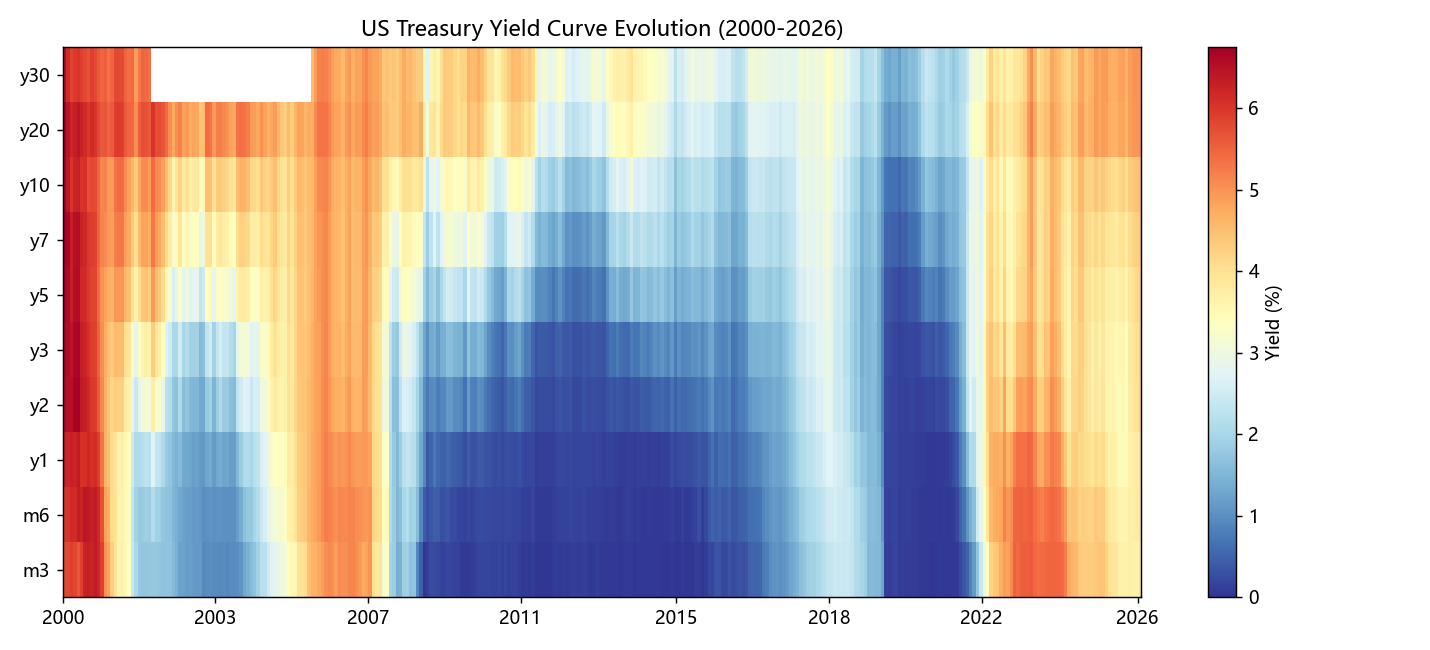
\includegraphics[width=0.9\textwidth]{f05_us_curve_heatmap.png}
\caption{美国国债收益率曲线演变（2000--2026）。颜色表示收益率水平。}
\label{fig:usheat}
\end{figure}

\begin{figure}[H]\centering
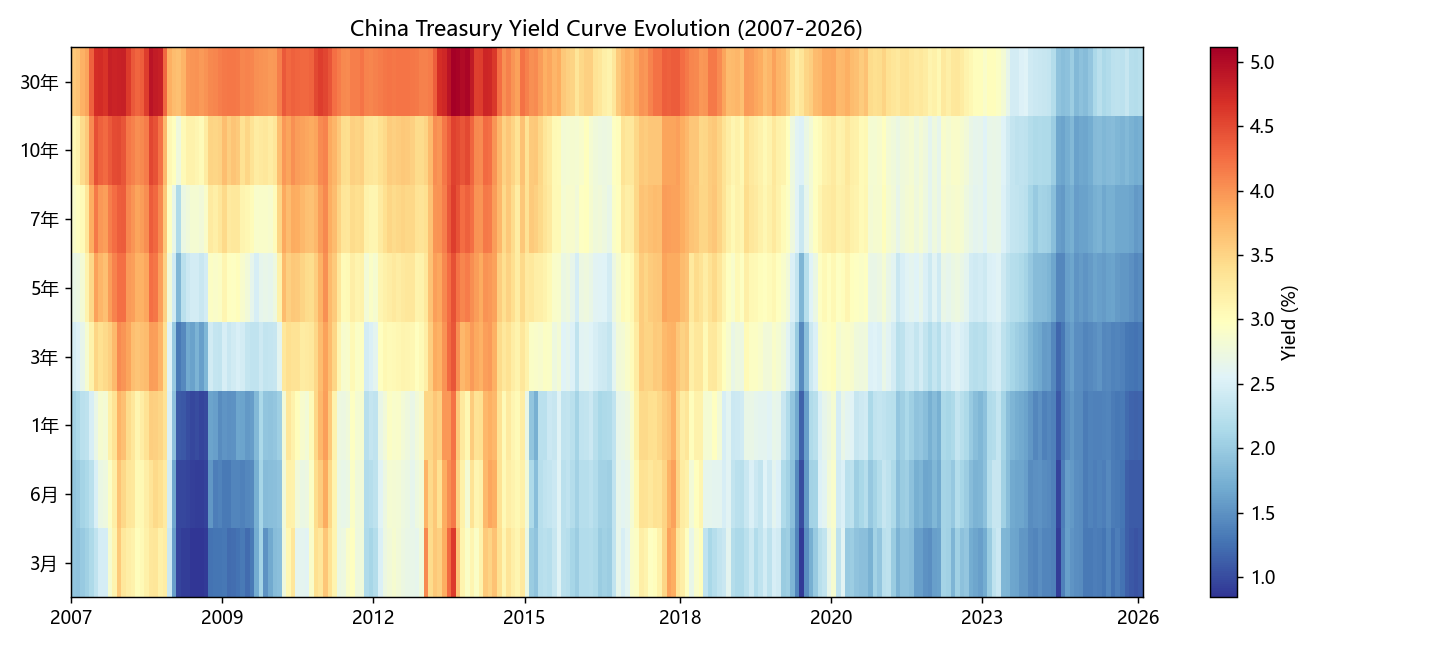
\includegraphics[width=0.9\textwidth]{f06_cn_curve_heatmap.png}
\caption{中国国债收益率曲线演变（2007--2026）。中枢更平稳，近年趋势性下移。}
\label{fig:cnheat}
\end{figure}

从热力图可读出两条重要信息：其一，美国曲线的"颜色带"在 2022--2023 年整体快速变暖（收益率全面抬升）并出现短端高于长端的倒挂，体现政策利率主导下的平移与翻转；其二，中国曲线的颜色变化更温和、近年整体转冷（收益率下移），反映宽松周期与"资产荒"。两图的视觉对比直观呈现了"美国曲线由政策周期剧烈驱动、中国曲线由基本面慢变量平稳下移"的差异。

曲线快照（图~\ref{fig:snap}）对比 2019、2022、2026 三个时点：美国 2022 年末曲线显著倒挂（短端高于长端），2026 年回归正斜率；中国曲线始终保持温和正斜率且整体下移。

\begin{figure}[H]\centering
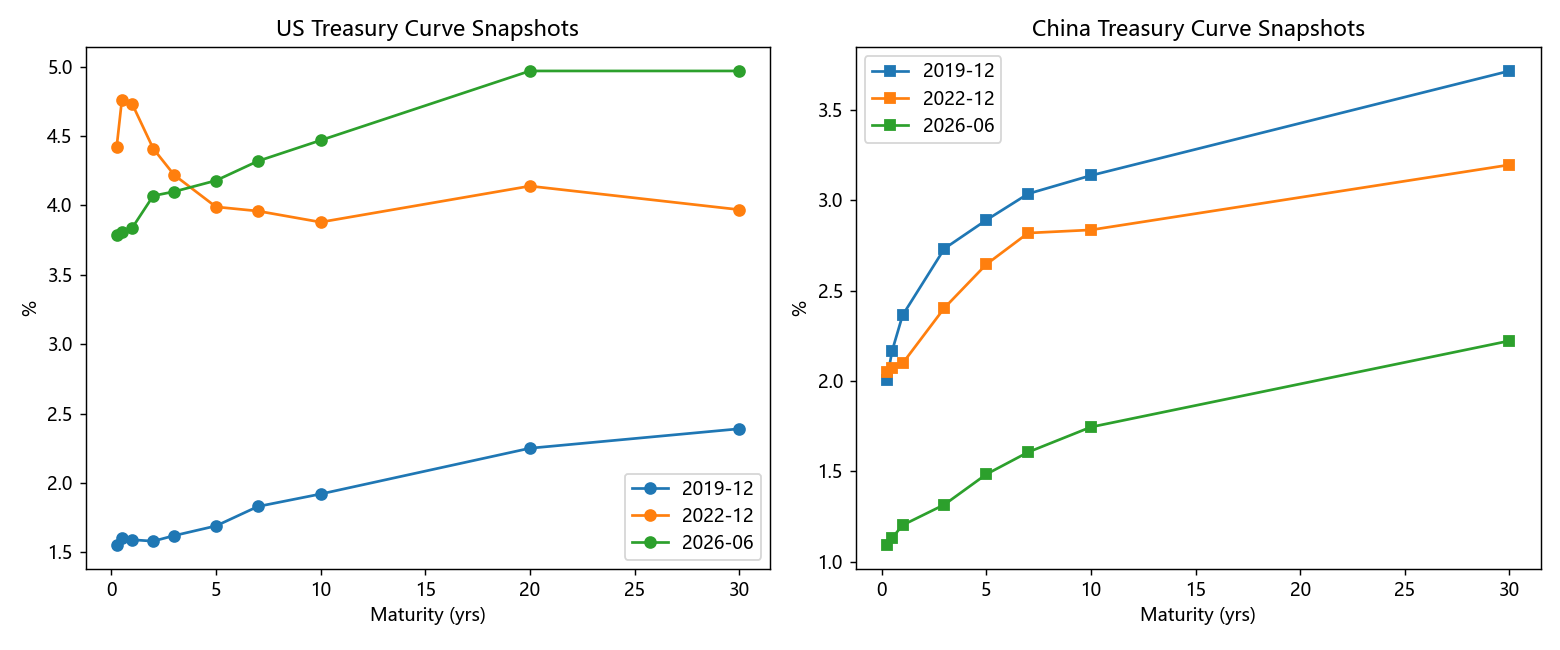
\includegraphics[width=0.95\textwidth]{f07_curve_snapshots.png}
\caption{中美收益率曲线快照对比（2019/2022/2026）。}
\label{fig:snap}
\end{figure}

期限利差（10Y--2Y）的周期见图~\ref{fig:termspread}。美国利差在 2022--2023 年深度倒挂（衰退预警的经典信号，\citealp{estrella1998}），而中国利差波动较小、未出现持续倒挂——反映两国曲线斜率由不同的政策与基本面驱动。

期限利差的差异具有宏观信号含义。在美国，10Y--2Y 利差是被广泛验证的衰退领先指标（\citealp{estrella1998}）：当市场预期政策利率将因经济走弱而下行时，短端高于长端，曲线倒挂。2022--2023 年的深度倒挂正是市场对"加息抗通胀$\to$经济放缓$\to$未来降息"路径的定价。在中国，曲线始终保持温和正斜率，一方面因政策利率本身处于低位、下行空间有限，另一方面因长端受"资产荒"与配置需求支撑。因此，简单套用"中国曲线是否倒挂"来判断衰退风险并不合适——两国曲线斜率的信息含量需在各自机制下解读。

\begin{figure}[H]\centering
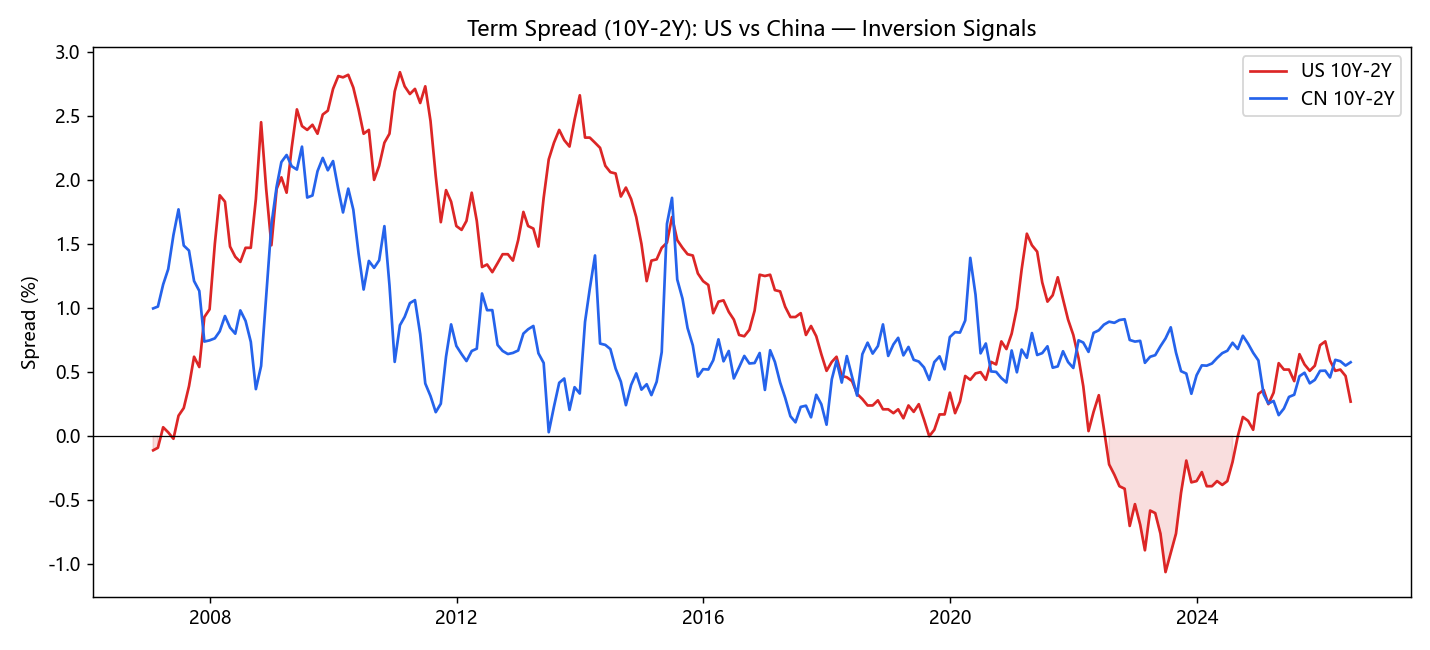
\includegraphics[width=0.92\textwidth]{f08_term_spread.png}
\caption{期限利差（10Y--2Y）：美国深度倒挂 vs 中国温和正斜率。}
\label{fig:termspread}
\end{figure}

\subsection{反应函数：泰勒规则对比（检验假说~\ref{h1}、\ref{h2}）}
表~\ref{tab:taylor} 报告两国含平滑泰勒规则的估计。美国（1990--2026，$n=435$）对核心 PCE 通胀的长期反应 $\phi_\pi=1.51>1$、对就业缺口 $\phi_{gap}=1.07$，$R^2=0.99$，满足泰勒原则；中国（2011--2026，$n=184$，被解释变量为 7 天 SHIBOR）$\phi_\pi=0.30<1$、$\phi_g=0.11$，$R^2=0.76$，价格规则明显较弱。

\begin{table}[H]
\centering
\caption{含平滑的泰勒规则估计（HAC 稳健 $t$ 值）}
\label{tab:taylor}
\small
\begin{tabular}{l cc | l cc}
\toprule
\multicolumn{3}{c|}{\textbf{美国（核心 PCE + 就业缺口）}} & \multicolumn{3}{c}{\textbf{中国（CPI + GDP 同比）}}\\
参数 & 系数 & $t$ & 参数 & 系数 & $t$ \\
\midrule
常数 & 0.008 & 0.16 & 常数 & 0.326 & 3.11 \\
通胀 $\pi$ & 0.030 & 1.28 & CPI $\pi$ & 0.073 & 1.98 \\
$-$就业缺口 & 0.022 & 2.34 & GDP $g$ & 0.026 & 1.74 \\
$i_{t-1}$ & 0.980 & 122.8 & $i_{t-1}$ & 0.755 & 10.43 \\
\midrule
$\rho$ & 0.980 & & $\rho$ & 0.755 & \\
$\phi_\pi$ & \textbf{1.51} & & $\phi_\pi$ & \textbf{0.30} & \\
$\phi_{gap}$ & 1.07 & & $\phi_g$ & 0.11 & \\
$R^2$ & 0.994 & & $R^2$ & 0.761 & \\
\bottomrule
\end{tabular}
\end{table}

图~\ref{fig:taylorus} 与图~\ref{fig:taylorcn} 分别给出两国规则的拟合。美国拟合几乎贴合实际（高 $R^2$ 部分源于高平滑），中国拟合误差更大，印证价格规则解释力较弱。

\begin{figure}[H]\centering
\begin{subfigure}{0.49\textwidth}\centering
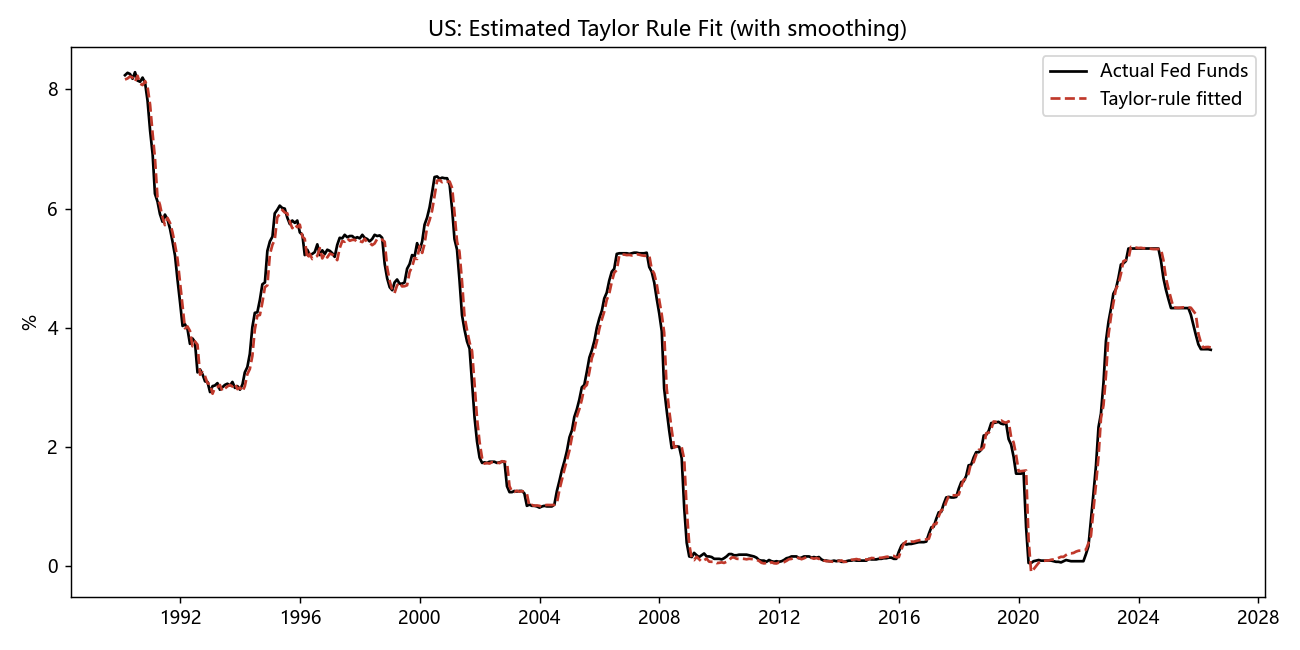
\includegraphics[width=\textwidth]{taylor_us_fit.png}
\caption{美国}\end{subfigure}
\begin{subfigure}{0.49\textwidth}\centering
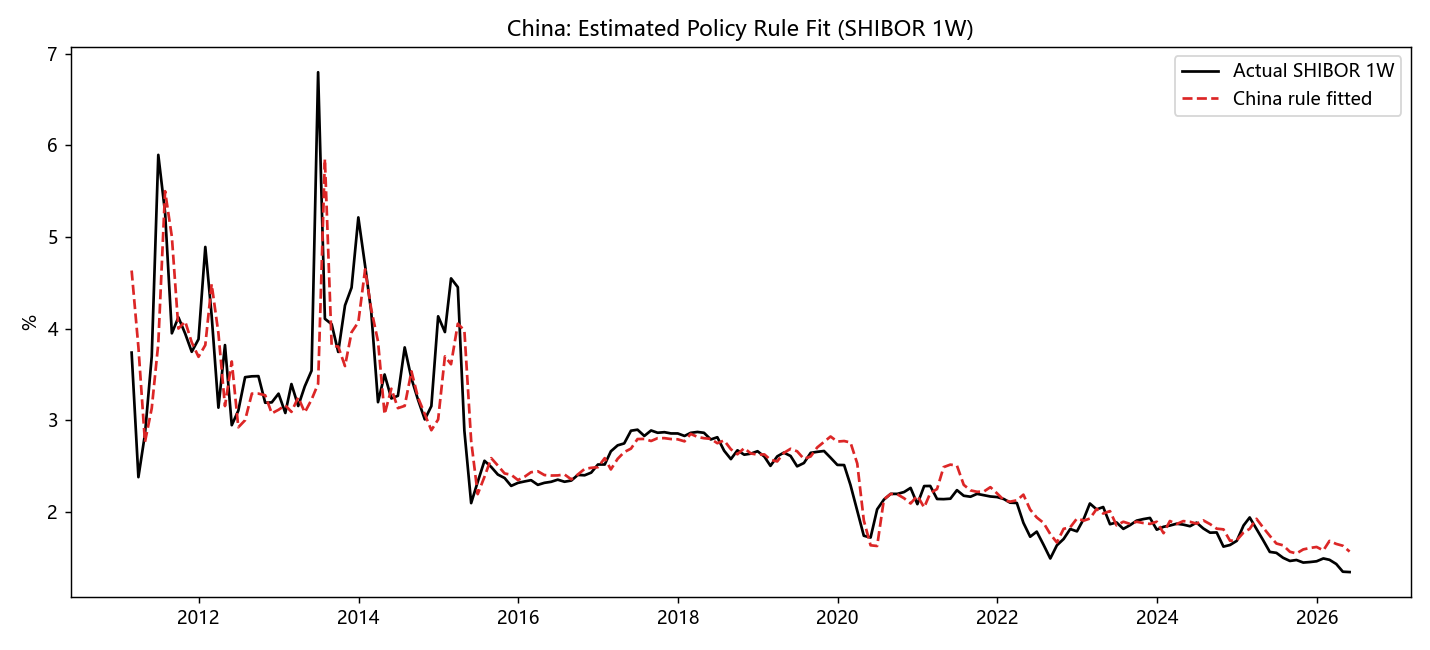
\includegraphics[width=\textwidth]{f04_taylor_cn_fit.png}
\caption{中国}\end{subfigure}
\caption{泰勒/政策规则拟合对比。}
\label{fig:taylorus}\label{fig:taylorcn}
\end{figure}

\textbf{解读。} (a) 美国对通胀长期反应超过 1，政策具备逆通胀稳定器性质（假说~\ref{h1} 美国侧成立）；(b) 中国对通胀反应显著小于 1（假说~\ref{h1} 中国侧成立），且整体拟合远低于美国（假说~\ref{h2} 成立）。这与制度事实一致：中国货币市场利率并非由单一通胀目标驱动，而是受增长、汇率、金融稳定与数量型工具共同影响，价格规则只是其中一维。需强调，美国 $\rho\approx0.98$ 极高，短期通胀系数本身不显著，长期 $\phi_\pi$ 由 $1/(1-\rho)$ 放大、对 $\rho$ 敏感（\citealp{rudebusch2002}），故应理解为"点估计层面满足泰勒原则"，但\emph{中美对比的定性结论是稳健的}。

从可信度（credibility）的角度看，反应函数拟合优度的差异还有更深的含义。一个高 $R^2$ 的反应函数意味着政策行为高度可预测，市场能据此形成稳定预期，从而使前瞻指引有效、长端定价"干净"。美国的高 $R^2$ 因此既是规则化的结果，也是可信度的体现。中国较低的 $R^2$ 并不意味着政策"无规律"，而是反映其反应函数维数更高、且包含难以被单一价格规则捕捉的数量维度与相机抉择成分。随着政策框架清晰化与沟通机制完善，可以预期中国反应函数的可预测性将逐步提升——这本身就是利率市场化"调得了"目标的应有之义。

\subsection{收益率曲线的主成分结构}
图~\ref{fig:pca} 给出中美收益率曲线的主成分分解。两国均呈现经典的"水平/斜率/曲率"三因子结构：美国前三个主成分的方差贡献率为 94.1\%、5.4\%、0.5\%；中国为 92.0\%、7.1\%、0.5\%。第一主成分（水平因子）主导曲线变动，两国相似；但中国斜率因子的相对占比更高，反映其曲线形态受短端流动性与政策节奏影响更大。

这一结果具有方法论含义：尽管两国利率决定机制在制度上差异显著，其收益率曲线的\emph{统计因子结构}却高度相似，均可由前两个因子解释逾 99\% 的方差。这说明无套利的期限结构规律（水平与斜率主导）在两国同样成立，机制差异更多体现在"因子如何被驱动"（美国由政策预期、中国由流动性与政策中枢）而非"因子结构本身"。对久期与曲线交易而言，这意味着可沿用统一的因子框架建模，但须以各自的宏观驱动变量解释因子变动。

\begin{figure}[H]\centering
\begin{subfigure}{0.49\textwidth}\centering
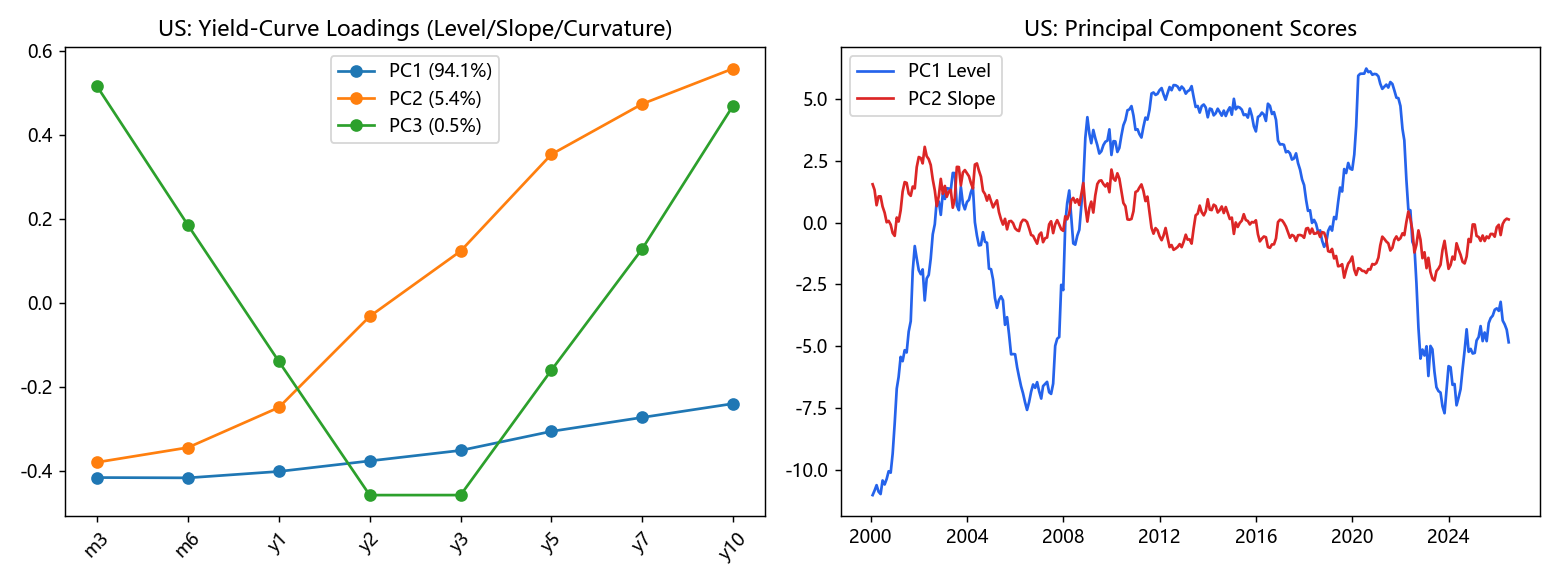
\includegraphics[width=\textwidth]{f09a_us_pca.png}
\caption{美国}\end{subfigure}
\begin{subfigure}{0.49\textwidth}\centering
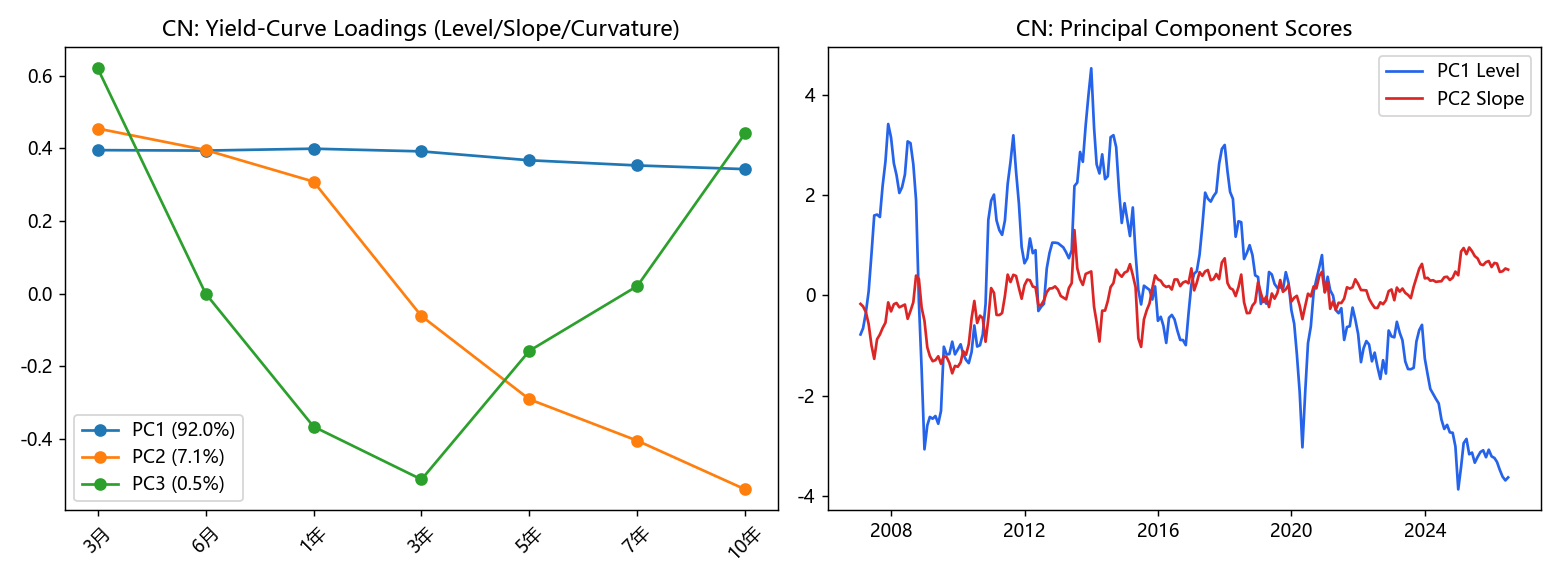
\includegraphics[width=\textwidth]{f09b_cn_pca.png}
\caption{中国}\end{subfigure}
\caption{收益率曲线主成分（载荷与得分）：水平/斜率/曲率。}
\label{fig:pca}
\end{figure}

\subsection{利率传导：误差修正模型（检验假说~\ref{h3}）}
表~\ref{tab:ecm} 与图~\ref{fig:ptbar} 报告传导估计。美国"联邦基金$\to$2 年"长期传导 0.82、即期 0.39，短端几乎是政策预期的镜像；中国"SHIBOR$\to$10 年"虽强协整（$p=0.001$），但即期传导仅 0.03、半衰期约 10 个月——货币市场短期波动几乎不立刻传到长端，长端更多反映对政策中枢与基本面的中期预期。LPR$\to$10 年长期传导 1.20，反映 2019 年 LPR 改革后政策中枢与债券利率的中期同向性（样本较短，需谨慎）。

\begin{table}[H]
\centering
\caption{利率传导误差修正模型估计}
\label{tab:ecm}
\small
\begin{tabular}{l ccccc}
\toprule
路径 & 长期 $b$ & 即期 $\gamma$ & 调整 $\lambda$ & 半衰期(月) & 协整 $p$ \\
\midrule
美国：联邦基金 $\to$ 2Y & \textbf{0.82} & \textbf{0.39} & $\approx 0$ & 长 & 0.038 \\
美国：联邦基金 $\to$ 10Y & 0.47 & 0.28 & $-0.07$ & 9.1 & 0.093 \\
中国：SHIBOR 1W $\to$ 10Y & 0.57 & \textbf{0.03} & $-0.06$ & 10.3 & \textbf{0.001} \\
中国：LPR 1Y $\to$ 10Y & 1.20 & 0.54 & $-0.12$ & 5.3 & 0.129 \\
\bottomrule
\end{tabular}
\end{table}

\begin{figure}[H]\centering
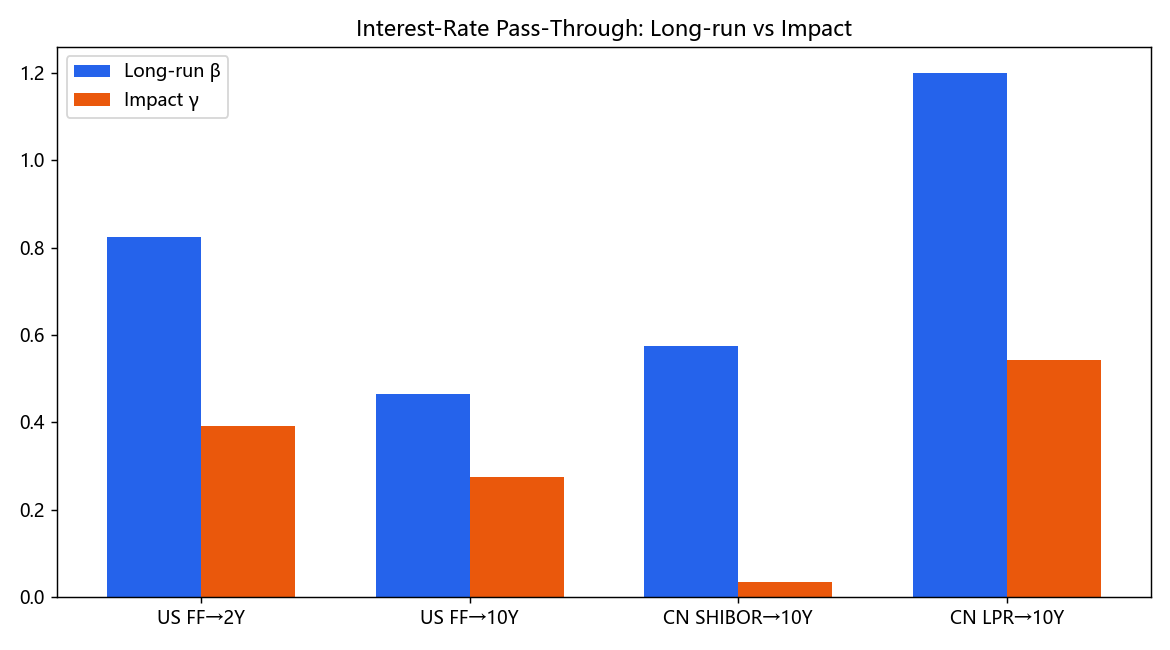
\includegraphics[width=0.8\textwidth]{f15_passthrough_bar.png}
\caption{利率传导：长期 $b$ 与即期 $\gamma$ 对比。中国 SHIBOR$\to$10Y 的即期传导极低。}
\label{fig:ptbar}
\end{figure}

\textbf{解读（假说~\ref{h3} 成立）。} 美国短端国债与政策利率高度一体、即时；中国货币市场与长端之间存在"强长期均衡 + 弱即期传导"的分层黏性，是双轨制下"短端高频扰动与长端慢变量并存"的量化表现。

\subsection{波动结构（检验假说~\ref{h4}）}
表~\ref{tab:vol} 对比 2011 年以来主要利率的水平与月度变动波动。中国货币市场利率的月度变动标准差（0.48）约为美国联邦基金（0.15）的三倍——因其由流动性供求实时出清，受缴税、跨季、外汇占款与投放节奏影响；而中国信贷基准 LPR 极黏（0.06）。反观美国，短端被行政利率牢牢钉住、波动最小，长端波动最大。两国"哪段利率最稳、哪段最活"恰好相反，是机制差异的直接指纹（假说~\ref{h4} 成立）。

这一"波动指纹"具有深刻的机制含义。在美国，政策利率由行政利率（IORB/ON RRP）直接钉住，故波动最小；市场化的长端则吸收了对未来政策路径与期限溢价的全部预期波动，故波动最大。在中国，恰恰相反：货币市场利率作为流动性出清的价格，承担了缴税、跨季、外汇占款与投放节奏的高频扰动；而 LPR 作为信贷定价基准，被赋予"稳定融资成本"的政策职能，故被刻意维持平稳。换言之，两国把"波动"分配给了利率曲线的不同位置——美国让市场化的长端承担波动、政策端保持稳定；中国让流动性出清的短端承担波动、信贷基准保持稳定。这种波动分配的差异，是两套机制在风险与信号传递上的不同设计选择。

\begin{table}[H]
\centering
\caption{利率水平与波动（2011--，月度）}
\label{tab:vol}
\small
\begin{tabular}{l ccccc}
\toprule
序列 & 均值\% & 标准差 & $\Delta$标准差 & 最小 & 最大 \\
\midrule
美国 联邦基金 & 1.56 & 1.85 & \textbf{0.152} & 0.05 & 5.33 \\
美国 10Y & 2.61 & 1.06 & 0.232 & 0.55 & 4.88 \\
中国 SHIBOR 1W & 2.63 & 0.93 & \textbf{0.478} & 1.34 & 6.80 \\
中国 10Y & 3.10 & 0.69 & 0.121 & 1.62 & 4.55 \\
中国 LPR 1Y & 4.08 & 0.75 & \textbf{0.057} & 3.00 & 5.77 \\
\bottomrule
\end{tabular}
\end{table}

\subsection{货币数量渠道：M2 与价格信号}
中国机制区别于美国的核心，是数量型工具与价格型工具并行。图~\ref{fig:m2} 对比 M1/M2 同比增速与 SHIBOR。M2 增速由历史均值约 13.7\% 降至 2026 年中的 8.6\%，反映货币条件的趋势性变化；价格信号（SHIBOR）与数量信号（M2 增速）并非一一对应，二者共同构成政策立场。图~\ref{fig:m2deep} 展示 M2 余额的快速扩张（货币深化），这是理解中国利率"水平偏低但社融对增长拉动边际递减"的背景。

数量与价格信号的协调，是中国机制的精髓，也是其难以被单一泰勒规则刻画的根本原因。在数量型框架下，央行可通过存款准备金率、再贷款与公开市场净投放直接调节流动性总量，价格（利率）只是流动性出清的结果之一。当数量工具承担主要调节职能时，货币市场利率对通胀的"反应"会被稀释，表现为估计中的低 $\phi_\pi$。随着利率市场化推进，价格信号的权重上升，但数量工具并未退出——这正是"双轨"的含义。因此，评估中国货币政策立场不能只看某一利率，而需综合价格（OMO/DR007/LPR）与数量（M2、社融、准备金率）的整体配置。这与美国"以单一政策利率概括立场"的范式形成鲜明对照。

\begin{figure}[H]\centering
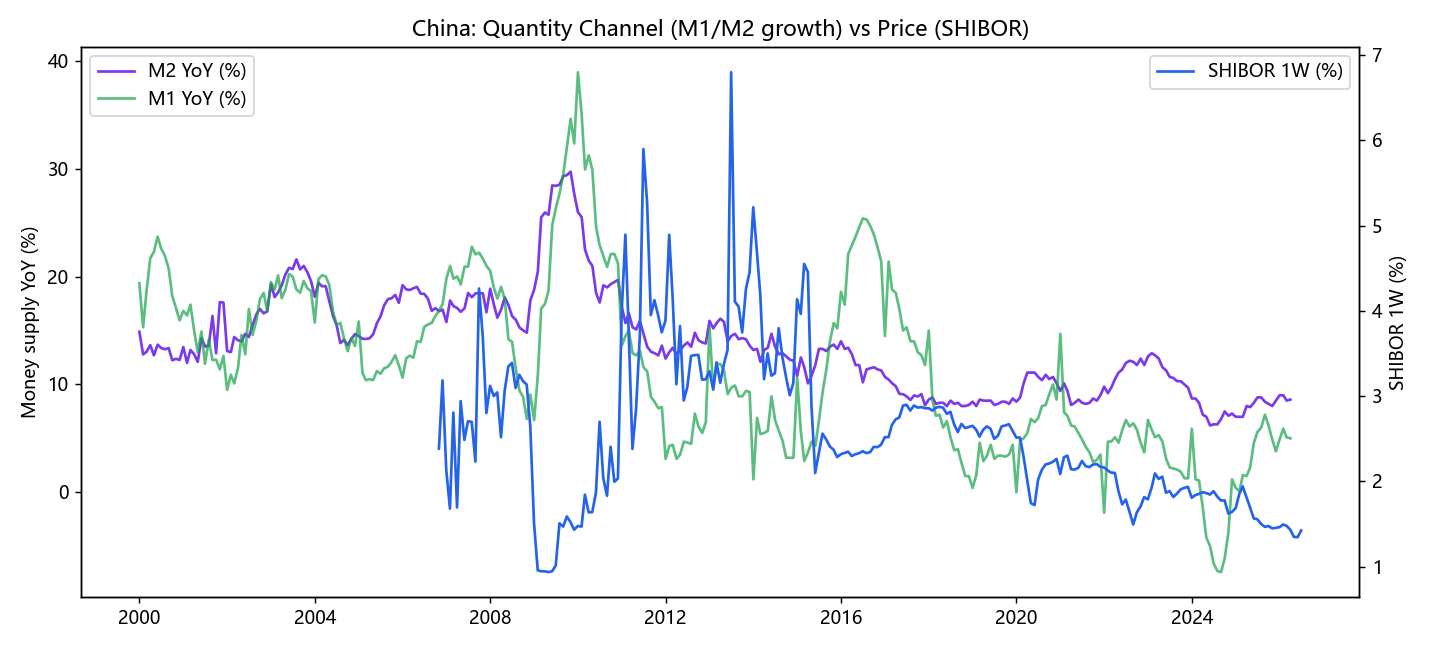
\includegraphics[width=0.9\textwidth]{f10_m2_vs_rate.png}
\caption{中国数量渠道（M1/M2 增速）与价格信号（SHIBOR）。}
\label{fig:m2}
\end{figure}

\begin{figure}[H]\centering
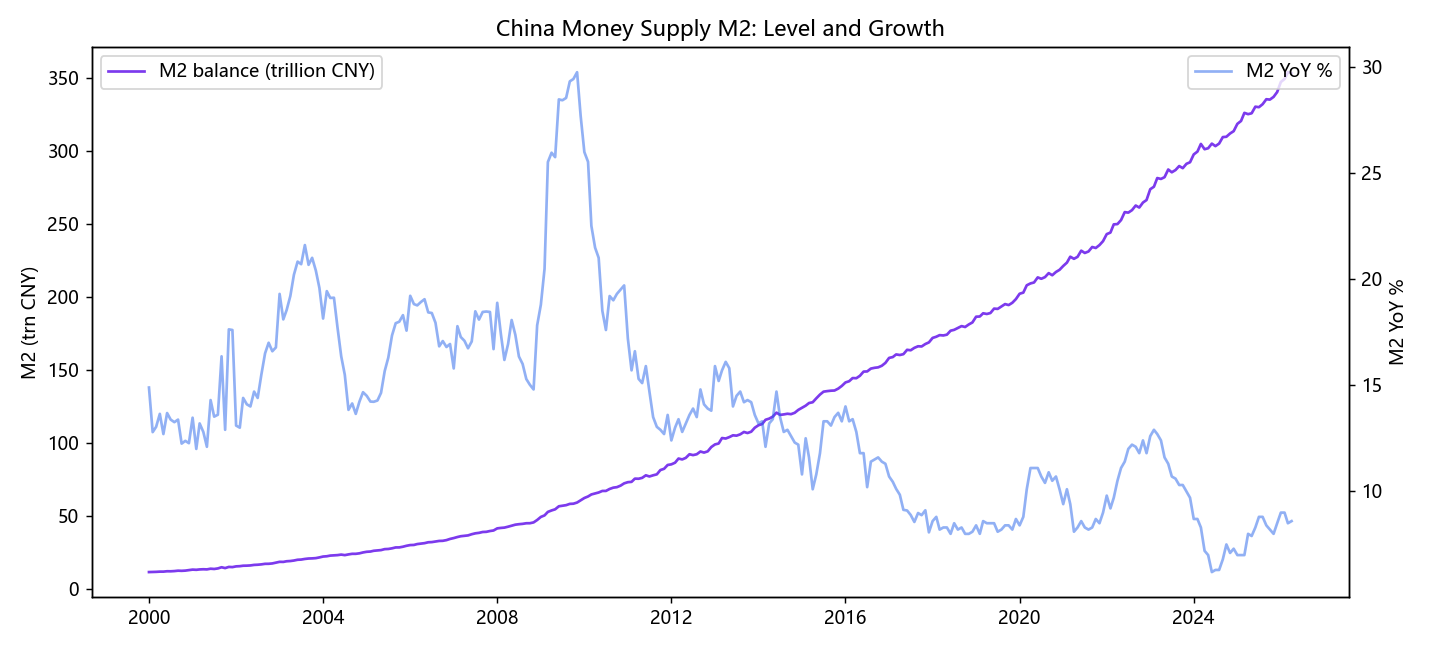
\includegraphics[width=0.9\textwidth]{f18_m2_deepening.png}
\caption{中国 M2 余额与增速：货币深化。}
\label{fig:m2deep}
\end{figure}

\subsection{实际利率与通胀：CPI 与 PPI 的差异}
图~\ref{fig:infl} 对比中美通胀。中国 CPI 长期温和，而 PPI 自 2022 年起持续为负（工业通缩），与美国 2021--2023 年的高通胀形成鲜明对照。图~\ref{fig:real} 给出事后实际 10 年期利率：以 PPI 平减，中国实际利率一度偏高（名义减负的 PPI）；以 CPI 平减则温和为正；美国实际利率在加息后显著转正（约 1.7\%）。通胀结构的差异，使两国"实际利率松紧"的判断必须采用各自的价格指数。

这一点对政策与配置都至关重要。中国 2022 年以来的 PPI 通缩意味着，以工业品价格平减的实际利率偏高，企业（尤其是制造业与上游）面临的真实融资成本并不低，这构成"名义利率已降、实体感受偏紧"的悖论，也是货币政策需要持续宽松的原因之一。而以 CPI 平减的实际利率温和，反映居民消费端价格平稳。美国则相反：高通胀阶段实际利率一度为负、金融条件实际宽松，加息后实际利率显著转正、政策真正进入限制性区间。因此，跨国比较"实际利率"时，必须明确使用何种价格指数，并理解 CPI 与 PPI 背后不同的经济含义——这是机制差异在"实际利率"这一关键变量上的具体体现。

\begin{figure}[H]\centering
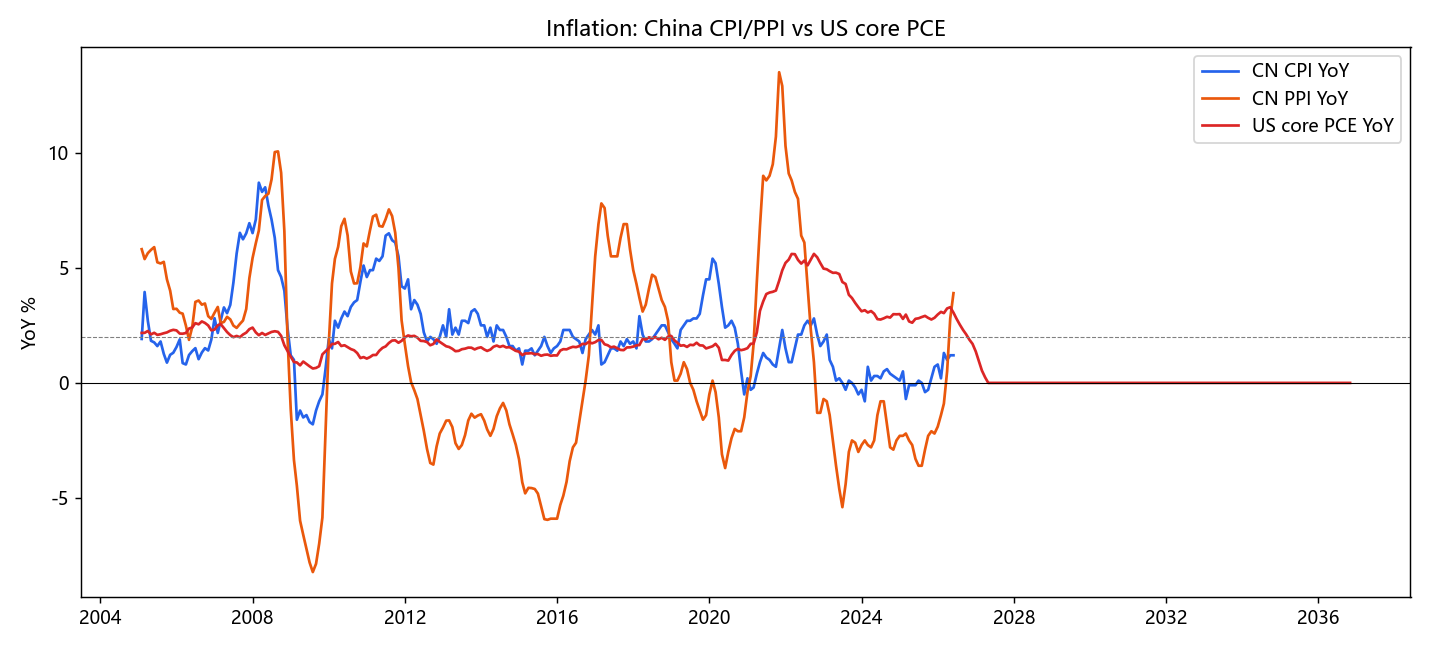
\includegraphics[width=0.9\textwidth]{f14_inflation.png}
\caption{通胀对比：中国 CPI/PPI vs 美国核心 PCE。中国 PPI 通缩与美国高通胀并存。}
\label{fig:infl}
\end{figure}

\begin{figure}[H]\centering
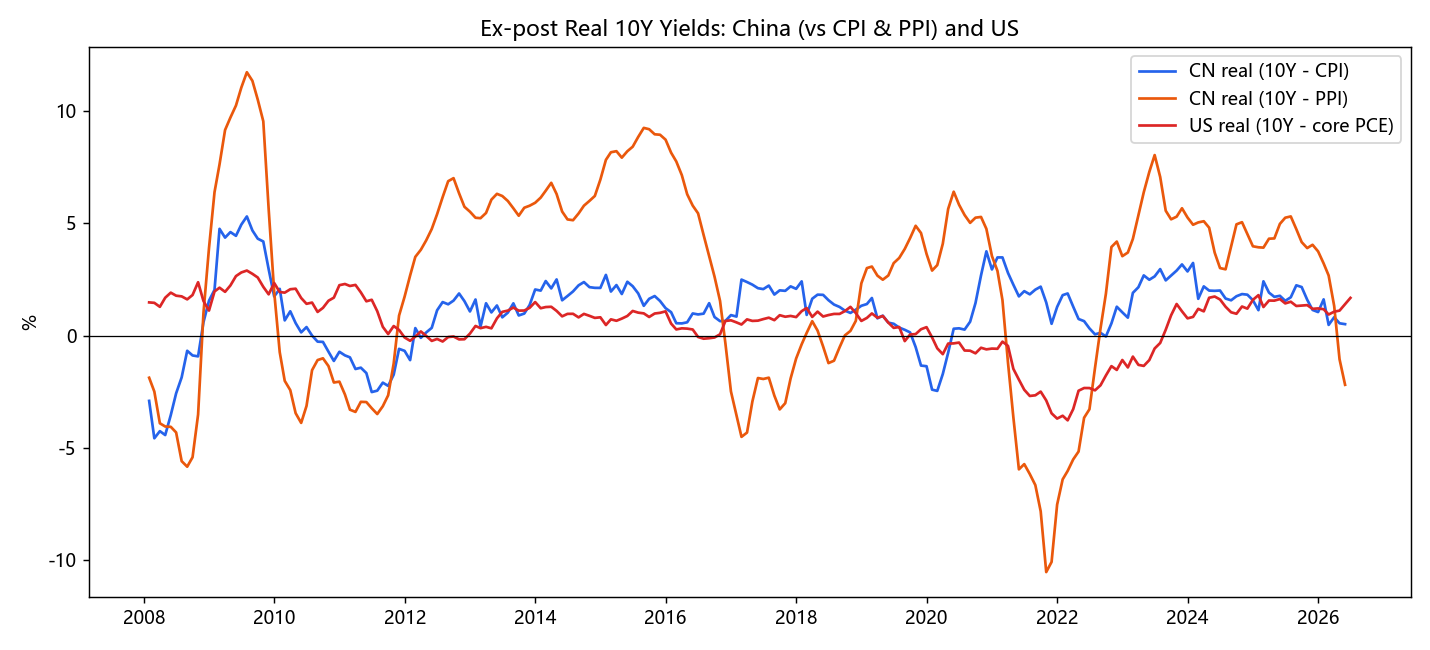
\includegraphics[width=0.9\textwidth]{f11_real_rates.png}
\caption{事后实际 10 年期利率：中国（对 CPI 与 PPI）与美国（对核心 PCE）。}
\label{fig:real}
\end{figure}

\subsection{中美联动、利差与溢出（检验假说~\ref{h5}）}
图~\ref{fig:spread} 给出中美 10 年期收益率与利差。两者水平相关系数为 $-0.18$（负），一阶差分相关 0.23（弱正），协整检验 $p=0.62$（不协整）；利差由历史均值 $+0.39\%$ 转为 2026 年中的深度倒挂。

\begin{figure}[H]\centering
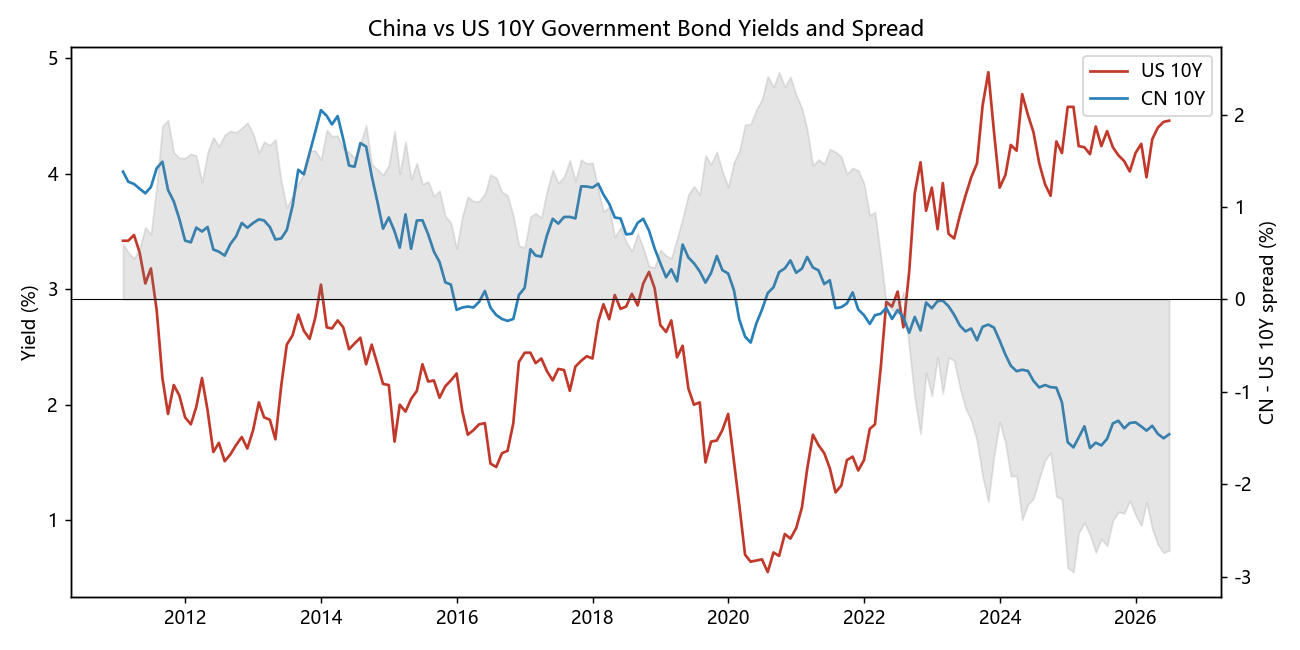
\includegraphics[width=0.92\textwidth]{spread_cn_us_10y.png}
\caption{中美 10 年期国债收益率与利差（CN$-$US）。由正利差转为深度倒挂。}
\label{fig:spread}
\end{figure}

图~\ref{fig:roll} 给出 $\Delta$US10Y 与 $\Delta$CN10Y 的滚动 24 个月相关，近年降至负值（期末约 $-0.24$），印证周期脱钩。但 Granger 因果检验显示：在月度差分上，\textbf{美国利率变动对中国存在单向短期溢出}（US$\to$CN，$p=0.020$ 显著；CN$\to$US，$p=0.291$ 不显著），与"全球金融周期"假说（\citealp{rey2015,miranda2020}）一致——即便水平脱钩，美债波动仍通过风险偏好与资本流动短期影响中债。

\begin{figure}[H]\centering
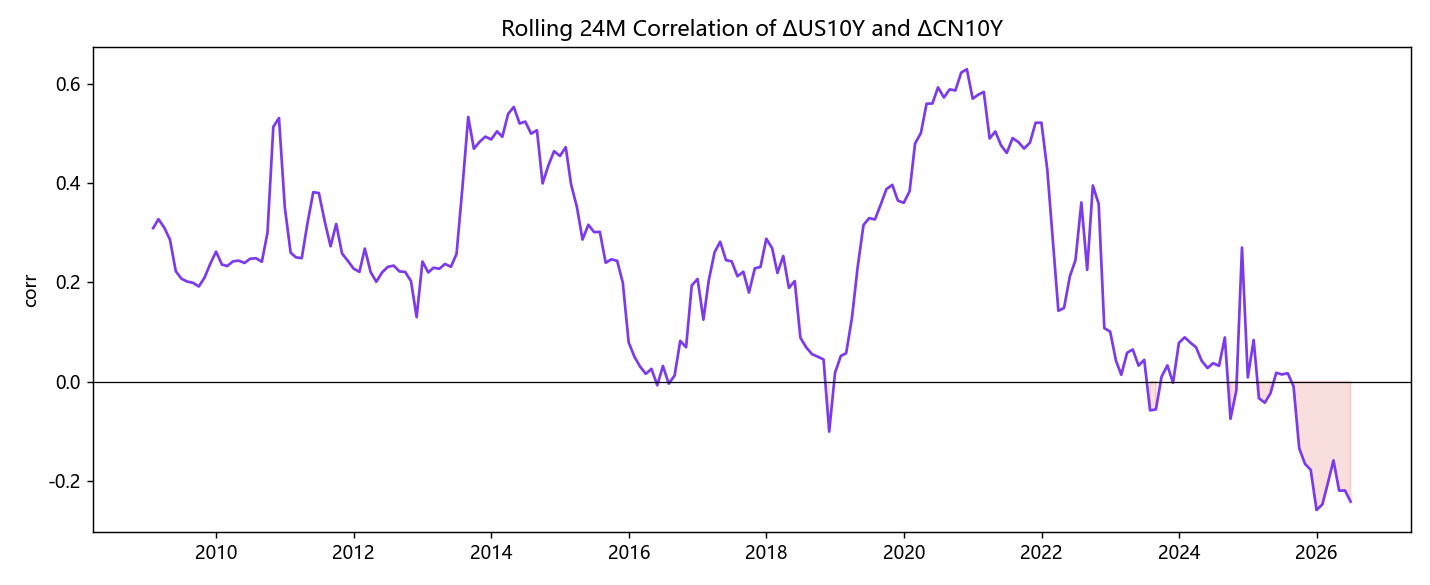
\includegraphics[width=0.9\textwidth]{f13_rolling_corr.png}
\caption{$\Delta$US10Y 与 $\Delta$CN10Y 的滚动 24 个月相关。近年转负。}
\label{fig:roll}
\end{figure}

\textbf{解读（假说~\ref{h5} 成立）。} 若中美利率被套利紧密绑定，两国长端应正相关并协整；数据显示水平负相关、不协整，证明在资本账户有管理的条件下，中国利率具备显著自主性，可在相当长时间内与美国周期背离。但短期溢出仍存在，说明自主性是\emph{程度问题}而非绝对隔离。

进一步地，从 UIP 视角看，中美利差 $i^{CN}-i^{US}$ 应等于预期汇率变动加风险与管制溢价 $\theta_t$。2022 年以来利差深度转负而人民币并未出现与利差对应幅度的趋势贬值，意味着 $\theta_t$（含资本流动管理与风险偏好）承担了相当部分的调整——这与"汇率由经常账户、预期与资本管理共同主导"的判断一致。换言之，机制差异不仅体现在利率的决定上，也通过 $\theta_t$ 改写了利差与汇率的经验关系，这对汇率对冲与跨境配置具有直接含义。

\subsection{利率走廊与基准体系}
图~\ref{fig:corridor} 展示中国货币市场利率（隔夜、1 周）与 LPR 的相对位置。货币市场利率在走廊内波动，LPR 作为信贷基准平滑下行，二者之间的"政策利率$\to$DR007$\to$LPR"传导构成中国价格型框架的骨架。

利率走廊的建设是中国价格型调控的关键一环。理想的走廊以常备借贷便利（SLF）利率为上沿、超额存款准备金利率为下沿，央行通过公开市场操作引导 DR007 在走廊内围绕政策利率（7 天逆回购利率）窄幅波动，从而稳定市场预期、降低利率波动。近年来，央行持续推进走廊收窄与政策利率体系的清晰化：强化 7 天逆回购利率作为主要政策利率的地位，淡化 MLF 的政策利率属性，并探索更对称、更窄的走廊。这些改革旨在提升价格信号的传导效率，使中国机制逐步向"以单一政策利率为锚、市场化传导"的方向演进。本文的传导实证（强协整但即期传导低）正反映了这一改革仍在进行、传导尚未完全顺畅的现实。

\begin{figure}[H]\centering
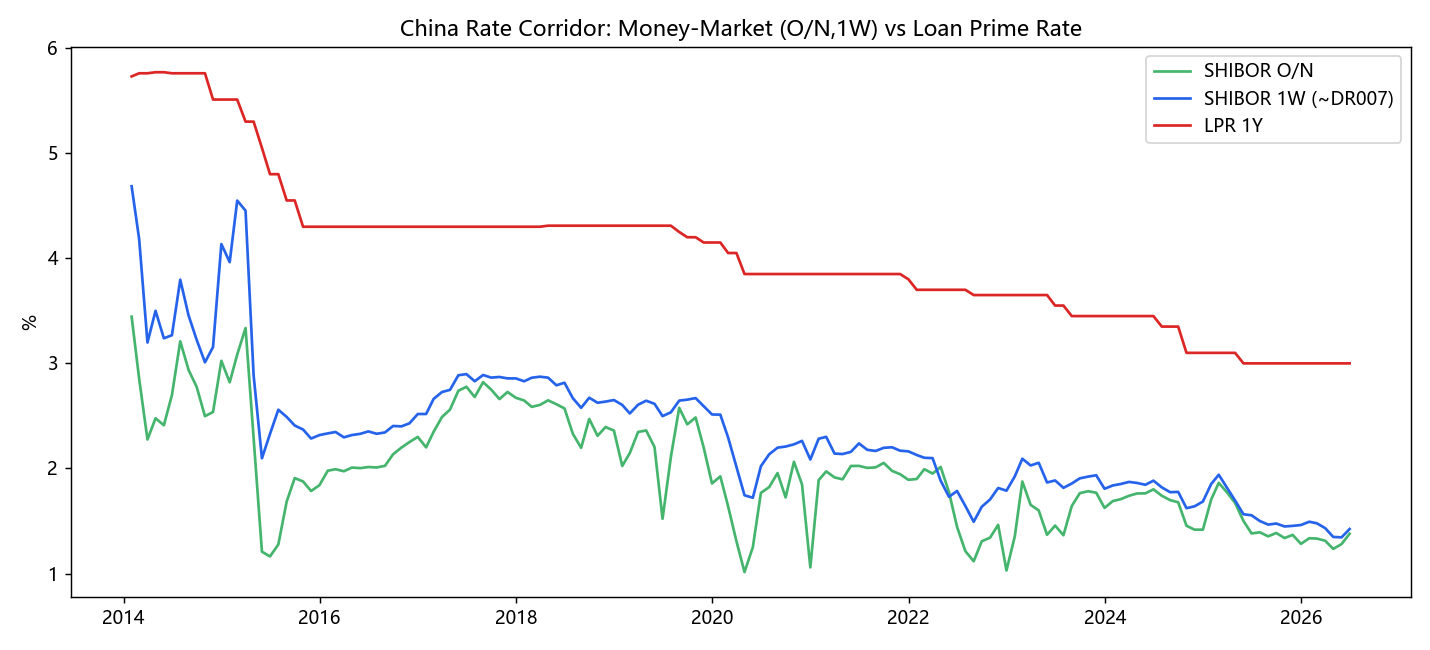
\includegraphics[width=0.9\textwidth]{f17_corridor.png}
\caption{中国利率走廊：货币市场利率（O/N、1W）与 LPR 1Y。}
\label{fig:corridor}
\end{figure}

% =====================================================================
\section{动态分析：脉冲响应与时变参数}

\subsection{货币政策冲击的脉冲响应（SVAR）}
为刻画政策利率冲击向长端的动态传导，我们对中美分别估计结构向量自回归（SVAR），采用递归（Cholesky）识别，变量次序为"通胀、实体（失业/增长）、政策利率变动、长端变动"，将政策利率冲击置于宏观变量之后。图~\ref{fig:svarus} 与图~\ref{fig:svarcn} 给出 10 年期收益率对一单位政策利率冲击的正交化脉冲响应。

\begin{figure}[H]\centering
\begin{subfigure}{0.49\textwidth}\centering
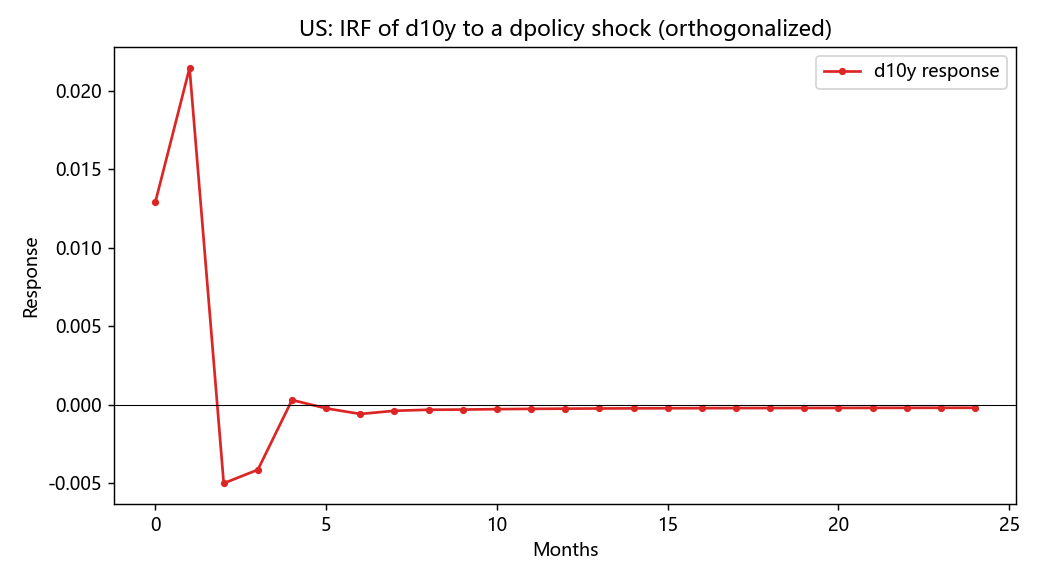
\includegraphics[width=\textwidth]{f20_svar_us.png}\caption{美国}\end{subfigure}
\begin{subfigure}{0.49\textwidth}\centering
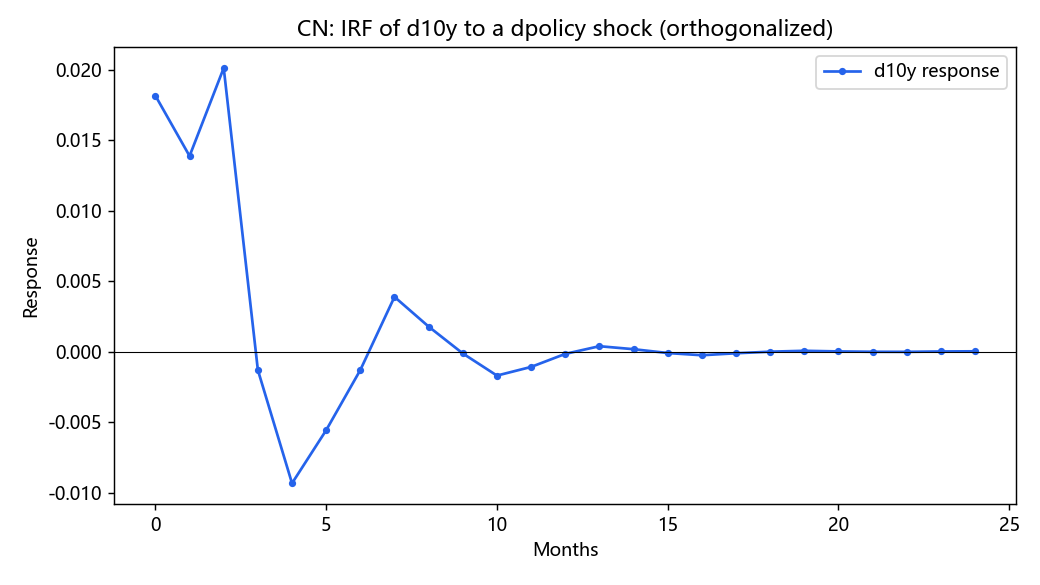
\includegraphics[width=\textwidth]{f21_svar_cn.png}\caption{中国}\end{subfigure}
\caption{10 年期收益率对政策利率冲击的脉冲响应（SVAR，24 个月）。}
\label{fig:svarus}\label{fig:svarcn}
\end{figure}

美国长端对政策冲击的响应更迅速、在前数月即显现并逐步收敛，反映市场对政策路径的快速定价；中国长端响应更平缓、峰值更靠后，与误差修正模型中"即期传导低、半衰期长"的结论一致。两国脉冲响应的形态差异，是传导速度差异在动态维度上的印证。

需要说明的是，SVAR 的识别依赖变量次序假设（Cholesky 递归），即假定通胀与实体经济在当期不受政策利率冲击的影响。这一假设对月度数据较为合理（实体变量的黏性高于金融变量），但脉冲响应的具体数值仍应被视为对动态形态的刻画而非精确的因果幅度。稳健性上，可改变变量次序、采用符号约束或高频识别（\citealp{miranda2020}）复核。本文关注的核心是\emph{形态对比}——美国响应更快收敛、中国响应更平缓滞后——这一定性结论对识别假设的微调并不敏感，且与误差修正模型的传导参数一致，互为印证。

\subsection{时变的通胀反应：滚动泰勒规则}
反应函数的参数并非恒定。图~\ref{fig:rolltaylor} 给出 60 个月滚动窗口估计的通胀长期反应 $\phi_\pi$。美国 $\phi_\pi$ 多数时期位于 1 之上（满足泰勒原则），并在高通胀的 2022--2023 年明显上行；中国 $\phi_\pi$ 长期低于 1，价格规则强度较弱且较稳定。这从时变角度再次支持假说~\ref{h1}。

\begin{figure}[H]\centering
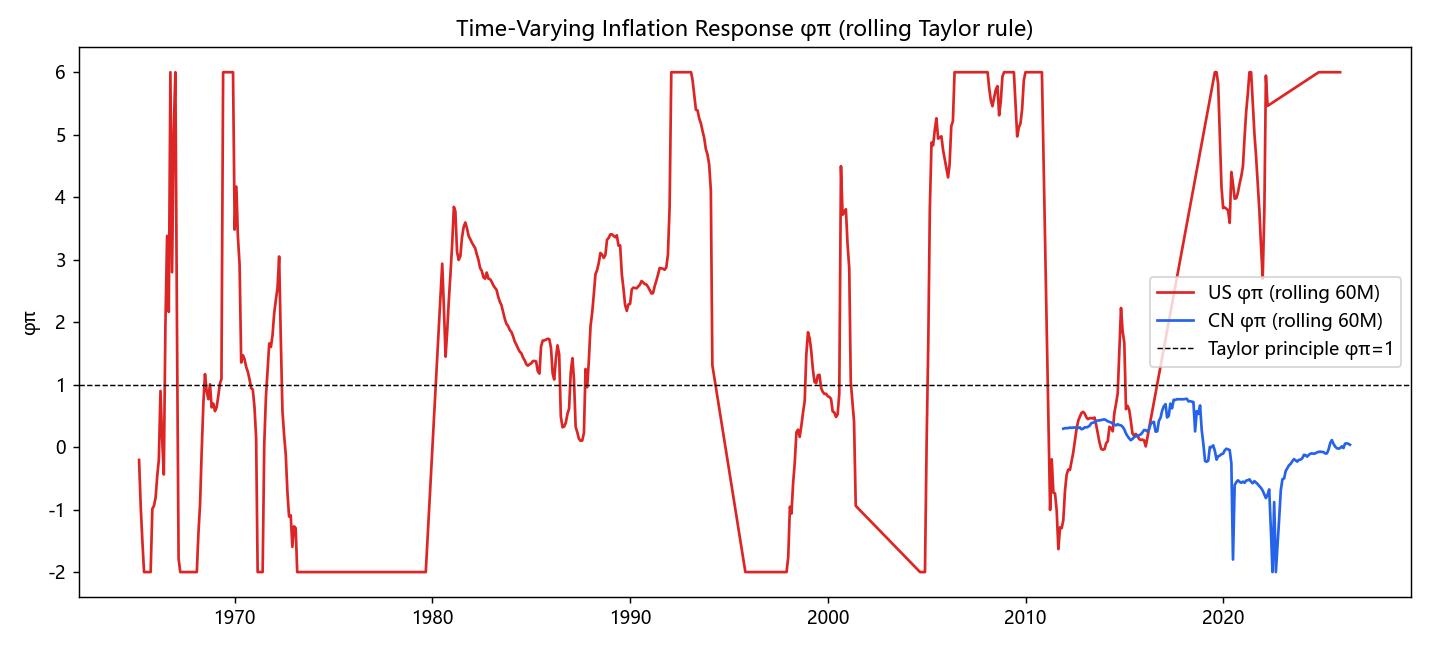
\includegraphics[width=0.9\textwidth]{f22_rolling_taylor.png}
\caption{时变通胀反应 $\phi_\pi$（60 个月滚动泰勒规则）。虚线为泰勒原则临界值 1。}
\label{fig:rolltaylor}
\end{figure}

\subsection{时变的跨国敏感度：滚动 Beta 与领先滞后}
图~\ref{fig:rollbeta} 给出 $\Delta$CN10Y 对 $\Delta$US10Y 的 36 个月滚动回归系数 $\beta$。该敏感度在不同时期波动，近年降至接近零，表明中债对美债变动的即期敏感度随中美周期脱钩而下降。图~\ref{fig:xcorr} 的领先滞后互相关显示，同期相关最强（$k=0$，约 0.23），并在美国领先方向（$k>0$）保留一定相关——与 Granger 检验"美国向中国单向短期溢出"相互印证。

\begin{figure}[H]\centering
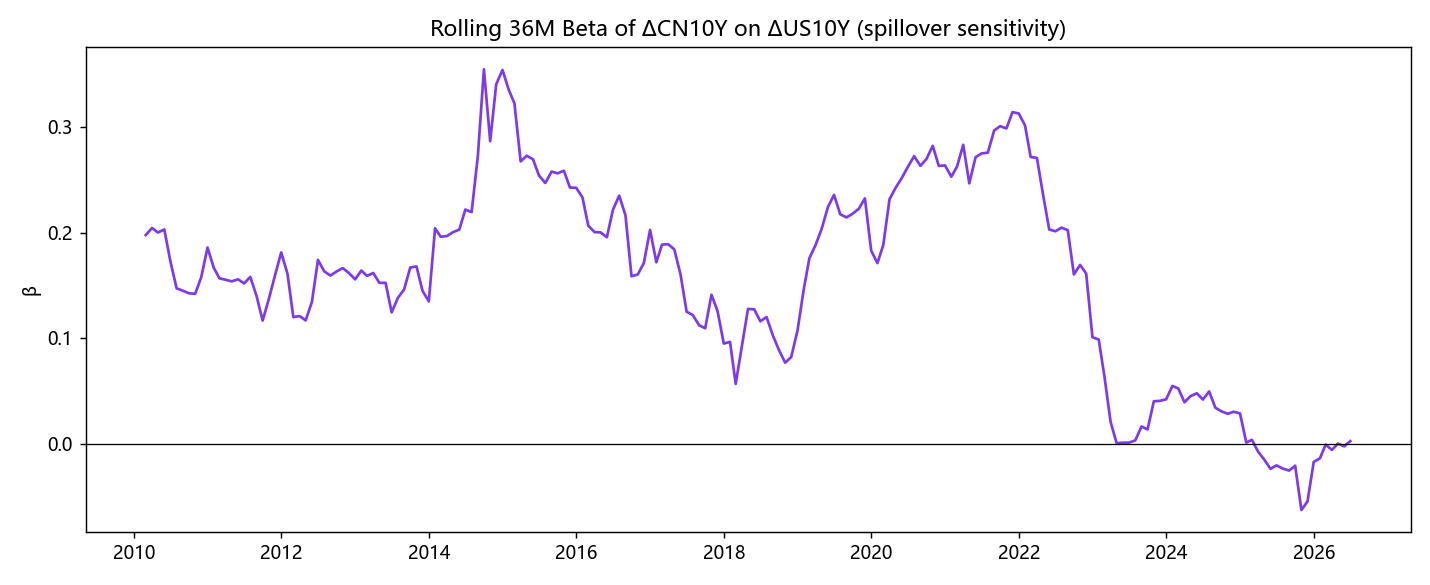
\includegraphics[width=0.9\textwidth]{f23_rolling_beta.png}
\caption{$\Delta$CN10Y 对 $\Delta$US10Y 的滚动 36 个月 $\beta$。近年趋近于零。}
\label{fig:rollbeta}
\end{figure}

\begin{figure}[H]\centering
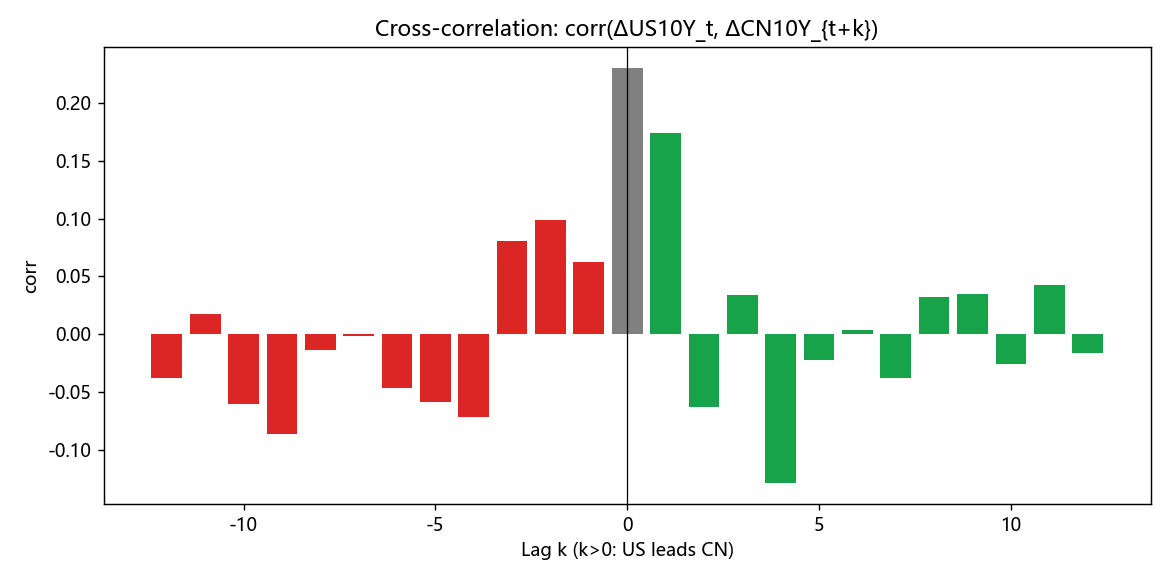
\includegraphics[width=0.82\textwidth]{f24_xcorr.png}
\caption{互相关 $\mathrm{corr}(\Delta\text{US10Y}_t,\Delta\text{CN10Y}_{t+k})$，$k>0$ 表示美国领先。}
\label{fig:xcorr}
\end{figure}

% =====================================================================
\section{机制差异的综合识别}
综合第 6 节，可把中美利率决定机制的差异归纳为五个可度量维度，见表~\ref{tab:summary}。

\begin{table}[H]
\centering
\caption{中美利率决定机制差异的量化刻画}
\label{tab:summary}
\small
\begin{tabular}{p{2.4cm} p{4.2cm} p{4.2cm} p{3.2cm}}
\toprule
\textbf{维度} & \textbf{美国} & \textbf{中国} & \textbf{量化证据} \\
\midrule
政策锚 & 单一通胀目标 + 就业 & 多目标 & $\phi_\pi$ 1.51 vs 0.30；$R^2$ 0.99 vs 0.76 \\
规则强度 & 满足泰勒原则、强价格规则 & 价格规则弱、数量价格双轨 & 反应函数 \\
传导速度 & 快、充分、市场化 & 慢、分层、黏滞 & 政策$\to$2Y 即期 0.39 vs SHIBOR$\to$10Y 即期 0.03 \\
波动指纹 & 短端最稳、长端最活 & 货币市场最活、信贷基准最稳 & $\Delta\sigma$：0.15 / 0.48 / 0.06 \\
跨国约束 & 嵌入全球套利 & 资本管理 $\to$ 自主性强 & 相关 $-0.18$、不协整；US$\to$CN 溢出 $p=0.02$ \\
\bottomrule
\end{tabular}
\end{table}

\textbf{一句话刻画：}美国 $=$ 单锚 $\cdot$ 强规则 $\cdot$ 快传导 $\cdot$ 强套利约束，利率是"市场对央行规则的连续定价"；中国 $=$ 多目标 $\cdot$ 弱价格规则 $\cdot$ 双轨数量价格 $\cdot$ 慢传导 $\cdot$ 强自主性，利率是"政策中枢 $+$ 流动性出清 $+$ 基本面预期"的分层合成。差异的根源在于：目标函数维数（单 vs 多）、工具组合（纯价格 vs 价格$+$数量）、金融结构（深市场/直接融资 vs 银行主导/分割市场）与资本账户开放度（高 vs 有管理）。

值得强调的是，这五个维度并非相互独立，而是构成一个\emph{自洽的制度组合}。一个银行主导、间接融资为主的金融体系，天然需要数量型工具直接调节信贷；高储蓄、有管理的资本账户为这一体系提供了相对独立的利率定价空间；多目标制则要求政策在增长、物价、汇率与金融稳定之间相机权衡，从而弱化了对单一通胀目标的机械反应。反观美国，深度市场、自由资本流动与单一明确使命，同样自洽地支撑了"强规则、快传导、市场定价"的体系。理解这一点很重要：中美利率机制的差异，不是某个单一制度选择的结果，而是一整套相互强化的制度安排的产物。这也意味着，机制的趋同将是一个渐进、系统性的长期过程，而非单一改革所能完成。

从动态演化的角度看，中国利率机制正沿着两条路径与"成熟价格型框架"靠拢：一是利率市场化的深化（存贷款利率上限放开、LPR 改革、走廊收窄、政策利率清晰化），二是金融市场的发展（债券市场扩容、衍生品工具完善、机构投资者壮大）。本文子样本估计中"价格规则权重上升、平滑系数趋近于 1"的特征，正是这一演化的统计痕迹。可以预期，随着改革推进，中国的价格规则强度（$\phi_\pi$）与传导效率（即期 $\gamma$）将逐步提升，但只要多目标制、银行主导结构与资本账户管理这三大制度特征仍然存在，中美机制就不会完全趋同，中国利率的相对自主性也将得以维持。这为长期的跨市场配置提供了一个稳定的判断基准。

% =====================================================================
\section{机制差异的深层成因}
第 7 节用五个维度刻画了"差异是什么"，本节进一步讨论"差异为何存在"，从金融结构、储蓄--投资、资本账户、财政--货币关系与中央银行使命五个层面给出经济学解释。

\subsection{金融结构：直接融资 vs 银行主导}
美国是直接融资主导的市场化金融体系，债券与股票市场深、广、流动性高，价格发现充分，政策利率的变化能迅速、完整地沿收益率曲线传导，并通过财富效应与市场化信贷影响实体。中国则是银行主导的间接融资体系，信贷在社会融资中占比高，银行负债端（存款）成本具有黏性，存款利率自律机制进一步平滑了利率波动。这解释了为何中国的信贷基准（LPR）极其黏滞、而货币市场利率却高频波动：前者承担"稳定信贷成本"的功能，后者承担"流动性出清"的功能，二者被刻意分置于不同的波动区间。金融结构因此是"价格规则弱、传导分层"的微观基础。

\subsection{储蓄--投资与自然利率}
利率的中枢由储蓄与投资的实际均衡（自然利率 $r^{*}$）锚定。中国长期高储蓄率支撑了较为充裕的可贷资金供给，而人口结构变化、地产投资回报下降与产能调整使投资需求边际放缓，二者共同压低了实际自然利率，构成中国名义利率水平中枢趋势性下移的实体基础（图~\ref{fig:cnheat} 中曲线近年整体下移与此一致）。美国的自然利率则受生产率、移民与财政赤字等因素影响，近年有所回升（\citealp{bauer2020} 强调 $r^{*}$ 的时变性对长端利率的影响）。两国自然利率的不同走向，是"中美利率水平脱钩"的实体根源，与货币政策操作层面的差异相互叠加。

\subsection{资本账户与三元悖论}
在蒙代尔--弗莱明的"三元悖论"框架下，固定汇率、资本自由流动与货币政策独立三者不可兼得。美国选择资本自由流动与货币独立，汇率浮动；其利率因此深度嵌入全球套利网络，UIP 偏离较小。中国选择保留相当程度的货币政策独立与汇率弹性，同时对资本账户进行宏观审慎管理；有管理的资本流动在 UIP 中形成"管制溢价" $\theta_t$，为国内利率提供了自主空间。本文实证中"中美 10 年期不协整、水平负相关"正是这一制度安排的统计表现；而"美国向中国的单向短期溢出"则说明在全球金融周期（\citealp{rey2015,miranda2020}）下，资本管理削弱但未消除外部冲击的传染。自主性因此是\emph{程度}而非\emph{有无}的问题。

\subsection{财政--货币关系与债券供给}
长端利率亦受国债供给与财政路径影响。美国财政赤字与国债存量的扩张，通过期限溢价对长端形成上行压力，并与货币政策路径共同决定曲线形态。中国的政府债务结构、地方债务化解与"资产荒"（高等级资产相对稀缺）则使长端国债需求旺盛、收益率承压下行。财政与货币的相对配置，是理解两国曲线斜率与期限溢价差异的重要补充维度。

\subsection{中央银行使命与目标维数}
最根本的差异在于中央银行的目标函数维数。美联储法定使命聚焦"物价稳定与充分就业"，目标维数低、可被单一价格规则较好近似，故 $\phi_\pi>1$ 的泰勒原则得以清晰识别。中国人民银行在多目标制下兼顾增长、就业、物价、国际收支、金融稳定与汇率，目标维数高，任一单一价格规则都只能解释其行为的一部分，这在统计上表现为较低的 $R^2$ 与较小的 $\phi_\pi$。目标维数的差异，是"规则强度"差异的制度根源，也决定了两国利率可被外部观察者"预测"的程度不同。

\subsection{小结}
综合而言，金融结构决定了传导的分层与黏性，储蓄--投资决定了利率中枢的走向，资本账户决定了跨国自主性，财政--货币关系决定了曲线形态，而中央银行使命的维数决定了规则强度。五者共同构成中美利率决定机制差异的深层成因，且彼此强化：多目标 $+$ 银行主导 $+$ 资本管理 $+$ 高储蓄，自洽地支撑了一个"弱价格规则、慢传导、强自主、低中枢"的中国利率体系，与美国"强规则、快传导、强套利、市场定价"的体系形成系统性对照。

% =====================================================================
\section{对大类资产配置的启示}

\subsection{中美利差与人民币汇率}
由于两国周期可独立（假说~\ref{h5}），传统"利差走阔$\to$人民币升值"的线性关系弱化。2022 年以来出现"深度负利差 $+$ 汇率由经常账户、预期与资本流动管理共同主导"的新格局。配置上应将\textbf{利差}与\textbf{风险溢价/资本流动}分离看待，而非以利差单一驱动汇率判断。

\subsection{久期策略的分国别定价}
中国长端由国内政策中枢与基本面慢变量决定、对货币市场扰动钝感（即期传导 0.03），故中债久期更受国内宽松周期与"资产荒"驱动；美债久期则对 FOMC 路径与期限溢价高度敏感。两者历史水平相关为负（$-0.18$），可作为分散化资产组合：在美债因加息承压时，中债可因国内宽松而走牛。

\subsection{贴现率与权益估值}
美股贴现率紧随美债曲线与实际利率（约 1.7\%）；A 股贴现率更受国内低而稳的 LPR/中债与风险偏好影响。中美无风险贴现锚不同步，意味着跨市场相对估值需各自以本币利率体系折现，不能简单套用同一贴现率。

\subsection{监测指标体系}
机制不同，领先指标不同：
\begin{itemize}[leftmargin=2em]
\item \textbf{美国}：核心 PCE、就业缺口、FOMC 点阵图与会议纪要、期限溢价（ACM）、SOFR 与国库券。
\item \textbf{中国}：OMO/MLF/LPR 政策中枢、DR007 与资金面、社融与 M2、存款准备金率、PPI 与实际利率、汇率与跨境资本流动。
\end{itemize}

\subsection{情景分析}
基于机制差异，可对中美政策组合的不同情景给出大类资产的方向性判断，见表~\ref{tab:scenario}。关键在于：两国利率由各自反应函数驱动，情景需\emph{分别}设定。

\begin{table}[H]
\centering
\caption{中美政策情景与大类资产方向（示意，非投资建议）}
\label{tab:scenario}
\small
\begin{tabular}{p{3.4cm} p{3.2cm} p{3.0cm} p{3.4cm}}
\toprule
\textbf{情景} & \textbf{中债} & \textbf{美债} & \textbf{人民币/权益} \\
\midrule
美降息 $+$ 中宽松（周期同向宽松） & 走牛（久期占优） & 走牛 & 利差收敛有限，权益贴现率双双下行利好 \\
美加息 $+$ 中宽松（当前态） & 走牛（自主宽松） & 承压 & 利差倒挂深化，汇率承压，需关注短期溢出 \\
美降息 $+$ 中收紧 & 承压 & 走牛 & 利差修复，人民币相对受益 \\
美加息 $+$ 中收紧（周期同向收紧） & 承压 & 承压 & 全球无风险利率上行，权益估值普遍承压 \\
\bottomrule
\end{tabular}
\end{table}

由实证可知，"美加息 $+$ 中宽松"情景下中债仍能走牛（即期传导仅 0.03、水平负相关），这是 2022--2024 年的现实写照；但须以滚动 $\beta$ 与 Granger 溢出监测阶段性相关上升的风险。

\subsection{风险管理含义}
机制差异对风险管理提出三点要求。其一，\textbf{相关性的时变性}。中美利率的相关并非恒定（图~\ref{fig:roll}、\ref{fig:rollbeta}），在常态下接近零甚至为负，但在全球风险事件中可能短暂上升，组合的分散化收益因此具有状态依赖性，需以滚动相关与滚动 $\beta$ 动态监测。其二，\textbf{尾部溢出}。Granger 检验显示美债向中债存在单向短期溢出，在美债剧烈波动（如加息预期重定价）时，中债可能阶段性同向，对冲策略应预留这一情形。其三，\textbf{汇率与利率的联合风险}。利差与汇率的关系因 $\theta_t$ 而非线性，跨境头寸需同时管理利率久期与汇率敞口，不可假设二者机械对冲。

\subsection{配置框架小结}
综上，建议采用"\textbf{双周期独立 $+$ 本币利率分别折现 $+$ 短期溢出对冲}"的框架：以各自的反应函数与基本面判断两国利率方向；以本币利率为各自资产的贴现锚；同时关注美债波动对中债的短期溢出（Granger $p=0.02$）以管理阶段性相关上升的风险。

% =====================================================================
\section{稳健性与局限}

\subsection{子样本稳健性：中国规则的阶段演变}
将中国样本分为数量型为主的 2011--2016 年与价格型推进的 2017--2026 年，分别估计政策规则，结果见表~\ref{tab:subsample}。2011--2016 年通胀长期反应 $\phi_\pi=0.06$、增长反应 $\phi_g=0.41$，规则以"稳增长"为主、对通胀几乎不反应；2017--2026 年回归的平滑系数 $\rho$ 趋近于 1，使长期系数在数值上不稳定（点估计被 $1/(1-\rho)$ 极度放大）。这一现象本身印证了 \citet{rudebusch2002} 的告诫：高度持续的政策利率使"长期反应系数"难以被精确识别。\textbf{稳健的定性结论}是：无论分期与否，中国价格规则对通胀的反应都显著弱于美国。

\begin{table}[H]
\centering
\caption{中国政策规则的子样本估计}
\label{tab:subsample}
\small
\begin{tabular}{l ccccc}
\toprule
样本 & $n$ & $R^2$ & $\rho$ & $\phi_\pi$ & $\phi_g$ \\
\midrule
2011--2016（数量型为主） & 71 & 0.49 & 0.56 & 0.06 & 0.41 \\
2017--2026（价格型推进） & 112 & 0.96 & $\approx 1.00$ & 不稳定 & 不稳定 \\
\bottomrule
\end{tabular}
\end{table}

\subsection{稳健性}
代码预留以下稳健性接口：(1) \textbf{子样本}：中国分 2011--2016（数量型为主）与 2017--2026（价格型推进）；美国分零利率下限（2009--2015、2020--2021）与非零利率期，零利率期可用影子利率（\citealp{wuxia2016}）替代。(2) \textbf{替代变量}：中国货币市场利率用 DR007/R007 替代 SHIBOR，政策利率用 OMO 7 天逆回购，通胀用 PPI/核心 CPI。(3) \textbf{方法}：以 ARDL 边界检验复核协整，以 SVAR 估计货币政策冲击脉冲响应，以 GMM 处理前瞻型规则的内生性（\citealp{clarida2000}）。

\subsection{局限}
其一，反应函数对平滑系数 $\rho$ 敏感，长期系数为点估计，不宜过度精确解读（\citealp{rudebusch2002}）。其二，中国政策利率体系处于改革进程中（MLF 属性变化、LPR 改革、走廊收窄），结构突变会影响参数稳定性。其三，LPR、GDP 等为低频/事件型数据，月度对齐采用前向填充，含近似。其四，资本账户管制溢价难以直接观测，本文以"不协整 $+$ 负相关"间接推断自主性。其五，本文使用事后通胀计算实际利率，与基于预期通胀的事前实际利率存在差异。

% =====================================================================
\section{结论}
本文用一组可复现的计量结果，把"中美利率决定机制的差异"从定性表述提升为可度量的参数对比。美国是"单锚—强规则—快传导—强套利约束"的市场化价格型机制（$\phi_\pi\approx1.51$、政策$\to$短端即期传导 0.39、嵌入全球套利）；中国是"多目标—弱价格规则—价格数量双轨—慢传导—强自主性"的转型期机制（$\phi_\pi\approx0.30$、SHIBOR$\to$长端即期传导 0.03、与美利率水平负相关且不协整，但存在美国向中国的单向短期溢出）。两套机制的差异，解释了当前中美利率深度倒挂却能长期共存的现实，并要求大类资产配置从"利差线性驱动"转向"双周期独立 $+$ 本币利率分别折现 $+$ 短期溢出对冲"的框架。

\subsection{政策与实践含义}
对政策制定者而言，本文的量化结果提示：中国价格型框架的传导仍存在"即期弱、长期强"的分层特征，深化利率市场化、收窄利率走廊、强化 7 天逆回购利率作为单一政策利率的锚定作用，有助于提升价格信号的传导效率与可预期性。对投资者而言，机制差异意味着不能以单一全球利率视角看待中美债券与权益，应建立分国别的反应函数监测与本币贴现框架，并对美债向中债的短期溢出保持风险对冲意识。

\subsection{研究展望}
本文存在若干可拓展方向。其一，引入影子利率（\citealp{wuxia2016,hamilton2012}）以更好刻画零利率下限时期的政策立场，并据此重估泰勒规则。其二，采用前瞻型规则与 GMM/工具变量（\citealp{clarida2000}）处理反应函数的内生性，区分政策对预期通胀与已实现通胀的反应。其三，运用高频货币政策冲击识别（\citealp{miranda2020}）量化中美溢出的因果强度。其四，将期限溢价（ACM）从长端利率中分离，比较两国"预期成分"与"风险成分"的相对贡献。其五，纳入时变参数（TVP-VAR）与结构突变检验，刻画中国机制随利率市场化改革的连续演变。这些拓展将进一步深化对中美利率决定机制差异的量化理解。

% =====================================================================
\clearpage
\begin{thebibliography}{99}
\small
\bibitem[Adrian et al.(2013)]{adrian2013} Adrian, T., Crump, R. K., \& Moench, E. (2013). Pricing the term structure with linear regressions. \emph{Journal of Financial Economics}, 110(1), 110--138.
\bibitem[Bernanke \& Blinder(1992)]{bernanke1992} Bernanke, B. S., \& Blinder, A. S. (1992). The federal funds rate and the channels of monetary transmission. \emph{American Economic Review}, 82(4), 901--921.
\bibitem[Campbell \& Shiller(1991)]{campbell1991} Campbell, J. Y., \& Shiller, R. J. (1991). Yield spreads and interest rate movements: A bird's eye view. \emph{Review of Economic Studies}, 58(3), 495--514.
\bibitem[Chen et al.(2018)]{chen2018} Chen, H., Chen, Q., \& Gerlach, S. (2018). The implementation of monetary policy in China: The interbank market and bank lending. \emph{Global Finance Journal}.
\bibitem[Clarida et al.(2000)]{clarida2000} Clarida, R., Gal\'i, J., \& Gertler, M. (2000). Monetary policy rules and macroeconomic stability: Evidence and some theory. \emph{Quarterly Journal of Economics}, 115(1), 147--180.
\bibitem[Diebold \& Li(2006)]{diebold2006} Diebold, F. X., \& Li, C. (2006). Forecasting the term structure of government bond yields. \emph{Journal of Econometrics}, 130(2), 337--364.
\bibitem[Engle \& Granger(1987)]{engle1987} Engle, R. F., \& Granger, C. W. J. (1987). Co-integration and error correction: Representation, estimation, and testing. \emph{Econometrica}, 55(2), 251--276.
\bibitem[Estrella \& Mishkin(1998)]{estrella1998} Estrella, A., \& Mishkin, F. S. (1998). Predicting U.S. recessions: Financial variables as leading indicators. \emph{Review of Economics and Statistics}, 80(1), 45--61.
\bibitem[Fernald et al.(2014)]{fernald2014} Fernald, J. G., Spiegel, M. M., \& Swanson, E. T. (2014). Monetary policy effectiveness in China: Evidence from a FAVAR model. \emph{Journal of International Money and Finance}, 49, 83--103.
\bibitem[Girardin et al.(2017)]{girardin2017} Girardin, E., Lunven, S., \& Ma, G. (2017). China's evolving monetary policy rule: From inflation-accommodating to anti-inflation policy. \emph{BIS Working Papers} No. 641.
\bibitem[G\"urkaynak et al.(2007)]{gurkaynak2007} G\"urkaynak, R. S., Sack, B., \& Wright, J. H. (2007). The U.S. Treasury yield curve: 1961 to the present. \emph{Journal of Monetary Economics}, 54(8), 2291--2304.
\bibitem[He \& Wang(2012)]{he2012} He, D., \& Wang, H. (2012). Dual-track interest rates and the conduct of monetary policy in China. \emph{China Economic Review}, 23(4), 928--947.
\bibitem[Litterman \& Scheinkman(1991)]{litterman1991} Litterman, R., \& Scheinkman, J. (1991). Common factors affecting bond returns. \emph{Journal of Fixed Income}, 1(1), 54--61.
\bibitem[Miranda-Agrippino \& Rey(2020)]{miranda2020} Miranda-Agrippino, S., \& Rey, H. (2020). U.S. monetary policy and the global financial cycle. \emph{Review of Economic Studies}, 87(6), 2754--2776.
\bibitem[Obstfeld et al.(2005)]{obstfeld2004} Obstfeld, M., Shambaugh, J. C., \& Taylor, A. M. (2005). The trilemma in history: Tradeoffs among exchange rates, monetary policies, and capital mobility. \emph{Review of Economics and Statistics}, 87(3), 423--438.
\bibitem[Orphanides(2001)]{orphanides2001} Orphanides, A. (2001). Monetary policy rules based on real-time data. \emph{American Economic Review}, 91(4), 964--985.
\bibitem[Porter \& Xu(2009)]{porter2010} Porter, N., \& Xu, T. (2009). What drives China's interbank market? \emph{IMF Working Paper} WP/09/189.
\bibitem[Rey(2015)]{rey2015} Rey, H. (2015). Dilemma not trilemma: The global financial cycle and monetary policy independence. \emph{NBER Working Paper} No. 21162.
\bibitem[Rudebusch(2002)]{rudebusch2002} Rudebusch, G. D. (2002). Term structure evidence on interest rate smoothing and monetary policy inertia. \emph{Journal of Monetary Economics}, 49(6), 1161--1187.
\bibitem[Sims(1980)]{sims1980} Sims, C. A. (1980). Macroeconomics and reality. \emph{Econometrica}, 48(1), 1--48.
\bibitem[Taylor(1993)]{taylor1993} Taylor, J. B. (1993). Discretion versus policy rules in practice. \emph{Carnegie-Rochester Conference Series on Public Policy}, 39, 195--214.
\bibitem[Woodford(2003)]{woodford2003} Woodford, M. (2003). \emph{Interest and Prices: Foundations of a Theory of Monetary Policy}. Princeton University Press.
\bibitem[Wu \& Xia(2016)]{wuxia2016} Wu, J. C., \& Xia, F. D. (2016). Measuring the macroeconomic impact of monetary policy at the zero lower bound. \emph{Journal of Money, Credit and Banking}, 48(2-3), 253--291.
\bibitem[易纲(2021)]{yigang2021} 易纲. (2021). 中国的利率体系与利率市场化改革. \emph{金融研究}, 总第 495 期.
\bibitem[孙国峰(2017)]{sunguofeng2017} 孙国峰, 蔡春春. (2017). 货币市场利率、流动性供求与中央银行流动性管理. \emph{经济研究}.
\bibitem[中国人民银行]{pboc} 中国人民银行. 《货币政策执行报告》（历期）.
\bibitem[Kim \& Wright(2005)]{kim2005} Kim, D. H., \& Wright, J. H. (2005). An arbitrage-free three-factor term structure model and the recent behavior of long-term yields and distant-horizon forward rates. \emph{FEDS Working Paper}.
\bibitem[Cochrane \& Piazzesi(2005)]{cochrane2005} Cochrane, J. H., \& Piazzesi, M. (2005). Bond risk premia. \emph{American Economic Review}, 95(1), 138--160.
\bibitem[Hamilton \& Wu(2012)]{hamilton2012} Hamilton, J. D., \& Wu, J. C. (2012). The effectiveness of alternative monetary policy tools in a zero lower bound environment. \emph{Journal of Money, Credit and Banking}, 44, 3--46.
\bibitem[Bauer \& Rudebusch(2020)]{bauer2020} Bauer, M. D., \& Rudebusch, G. D. (2020). Interest rates under falling stars. \emph{American Economic Review}, 110(5), 1316--1354.
\bibitem[Coibion \& Gorodnichenko(2012)]{coibion2012} Coibion, O., \& Gorodnichenko, Y. (2012). Why are target interest rate changes so persistent? \emph{American Economic Journal: Macroeconomics}, 4(4), 126--162.
\bibitem[Stock \& Watson(2001)]{stock2001} Stock, J. H., \& Watson, M. W. (2001). Vector autoregressions. \emph{Journal of Economic Perspectives}, 15(4), 101--115.
\bibitem[Taylor \& Williams(2009)]{taylor2009} Taylor, J. B., \& Williams, J. C. (2009). A black swan in the money market. \emph{American Economic Journal: Macroeconomics}, 1(1), 58--83.
\bibitem[Mishkin(2007)]{mishkin2007} Mishkin, F. S. (2007). \emph{The Economics of Money, Banking, and Financial Markets}. Pearson.
\bibitem[Ma et al.(2013)]{ma2013} Ma, G., Yan, X., \& Liu, X. (2013). China's evolving reserve requirements. \emph{Journal of Chinese Economic and Business Studies}, 11(2), 117--137.
\end{thebibliography}

% =====================================================================
\clearpage
\appendix
\section{复现说明}
全部数据与结果可一键复现：
\begin{verbatim}
pip install -r code/requirements.txt
# 1) 抓取数据（FRED 免 key；Tushare 需 token；akshare 公开接口）
export TS_TOKEN=<your_tushare_token>   # 或写入 code/ts_token.txt（已 gitignore）
python code/data_fetch.py
python code/tushare_fetch.py
# 2) 计量与作图
python code/analysis.py     # 泰勒规则/ECM/协整/波动 -> report/results.*
python code/analysis2.py    # 曲线/PCA/M2/实际利率/Granger -> figures/*
# 3) 编译论文
cd report && latexmk -xelatex paper.tex
\end{verbatim}

\section{方法论补充推导}

\subsection{泰勒规则的目标函数推导}
设中央银行最小化二次损失 $L_t = (\pi_t-\pi^{*})^2 + \omega\, x_t^2$，对名义利率 $i_t$ 一阶条件结合总需求（IS）与总供给（菲利普斯曲线）关系，可导出最优利率为通胀缺口与产出缺口的线性函数，即泰勒规则的形式 $i_t^{*} = c + \phi_\pi(\pi_t-\pi^{*}) + \phi_x x_t$。加入对利率剧烈变动的厌恶（平滑动机）$\theta(i_t-i_{t-1})^2$，最优解变为实际利率向目标利率的部分调整：$i_t = (1-\rho) i_t^{*} + \rho\, i_{t-1}$，即式~\eqref{eq:taylor}。泰勒原则 $\phi_\pi>1$ 保证名义利率上行幅度超过通胀，实际利率上升以抑制通胀，从而排除自我实现的通胀--通缩螺旋。

\subsection{两步误差修正模型}
若 $m_t,p_t$ 均为 $I(1)$ 且协整，则存在平稳的线性组合 $u_t=m_t-a-bp_t\sim I(0)$。Granger 表示定理保证存在等价的误差修正表示 $\Delta m_t = \gamma\Delta p_t + \lambda u_{t-1}+e_t$，其中 $\lambda<0$ 为向长期均衡回归的速度。第一步 OLS 估计协整向量（超一致），第二步以残差滞后项作为误差修正项估计短期动态。偏离的半衰期由 $(1+\lambda)^h=0.5$ 解得 $h=\ln 0.5/\ln(1+\lambda)$。

\subsection{收益率曲线主成分}
对中心化收益率矩阵 $Y_c$ 做奇异值分解 $Y_c=U\Sigma V^\top$，第 $k$ 个右奇异向量 $v_k$ 为载荷，主成分得分为 $Y_c v_k$，方差贡献率 $\sigma_k^2/\sum_j\sigma_j^2$。经验上 $v_1$ 各期限同号近似平行（水平），$v_2$ 短长端反号（斜率），$v_3$ 中段与两端反号（曲率）。

\subsection{SVAR 的递归识别}
对约简式 VAR $Y_t=\sum A_j Y_{t-j}+\varepsilon_t$（$\mathrm{Var}(\varepsilon_t)=\Sigma$），令 $\Sigma=PP^\top$ 为 Cholesky 分解，结构冲击 $\eta_t=P^{-1}\varepsilon_t$ 相互正交。变量次序蕴含同期因果的下三角约束：排在前的变量（通胀、实体）当期不受排在后的政策冲击影响，而政策利率冲击可当期影响其后的长端。脉冲响应 $\partial Y_{t+h}/\partial \eta_t$ 由 $A_j$ 与 $P$ 递推得到。

\subsection{Granger 因果}
在双变量 VAR 中，若将 $x$ 的滞后项加入 $y$ 的方程能显著降低残差平方和（$F$ 检验拒绝零假设），则称 $x$ Granger 引致 $y$。本文对 $\Delta$US10Y 与 $\Delta$CN10Y 双向检验，发现仅 US$\to$CN 显著（$p=0.02$），即美国利率变动有助于预测中国利率变动，反向不成立。

\section{补充统计表}

\subsection{描述统计（2011--，月度）}
\begin{table}[H]\centering\caption{主要变量描述统计}\small
\begin{tabular}{l ccccc}
\toprule
变量 & 均值 & 标准差 & 最小 & 最大 & $n$ \\
\midrule
美国 联邦基金 & 1.56 & 1.85 & 0.05 & 5.33 & 185 \\
美国 10Y & 2.61 & 1.06 & 0.55 & 4.88 & 186 \\
美国 核心PCE 同比 & 1.44 & 1.47 & 0.00 & 5.61 & 310 \\
中国 SHIBOR 1W & 2.63 & 0.93 & 1.34 & 6.80 & 186 \\
中国 10Y & 3.10 & 0.69 & 1.62 & 4.55 & 186 \\
中国 LPR 1Y & 4.08 & 0.75 & 3.00 & 5.77 & 186 \\
\bottomrule
\end{tabular}\end{table}

\subsection{单位根检验（ADF，原序列 $p$ 值）}
\begin{table}[H]\centering\caption{ADF 单位根检验}\small
\begin{tabular}{l c l}
\toprule
序列 & ADF $p$ 值 & 结论 \\
\midrule
美国 联邦基金 & 0.035 & 接近平稳 \\
美国 10Y & 0.495 & 非平稳（$I(1)$） \\
中国 SHIBOR 1W & 0.184 & 非平稳（$I(1)$） \\
中国 10Y & 0.629 & 非平稳（$I(1)$） \\
\bottomrule
\end{tabular}\end{table}
多数利率序列为 $I(1)$，故对"政策$\to$市场"采用协整/误差修正框架，避免伪回归。

\section{术语与变量对照}
\begin{description}[leftmargin=2.2cm,style=nextline]
\item[EFFR] 联邦基金有效利率，美国短端政策利率的市场实现值。
\item[IORB] 准备金余额利率，地板系统下的行政利率工具。
\item[ON RRP] 隔夜逆回购便利利率，利率走廊下沿。
\item[OMO] 公开市场操作；中国以 7 天逆回购利率为主要政策利率。
\item[MLF] 中期借贷便利，1 年期，2024 年后政策利率属性弱化。
\item[LPR] 贷款市场报价利率，中国贷款定价基准（1 年/5 年期）。
\item[DR007] 银行间存款类机构 7 天质押式回购利率，货币市场基准（本文以 SHIBOR 1 周为可复现代理）。
\item[SHIBOR] 上海银行间同业拆放利率。
\item[RRR] 存款准备金率，数量型工具。
\item[$\phi_\pi,\phi_x$] 泰勒规则中对通胀缺口与产出/就业缺口的长期反应系数。
\item[$\rho$] 利率平滑系数。
\item[$b,\gamma,\lambda$] 误差修正模型中的长期传导、即期传导与调整速度。
\item[PCE / 核心 PCE] 个人消费支出价格指数（剔除食品能源），美联储首选通胀指标。
\item[PPI] 生产者价格指数；中国 2022 年后持续为负（工业通缩）。
\item[UIP / CIP] 非抛补/抛补利率平价。
\end{description}

\section{核心结果数值索引}
反应函数：美 $\phi_\pi=1.51$、$R^2=0.99$；中 $\phi_\pi=0.30$、$R^2=0.76$。传导：美 FF$\to$2Y 即期 0.39/长期 0.82；中 SHIBOR$\to$10Y 即期 0.03/长期 0.57（协整 $p=0.001$）。曲线 PCA：美 94.1/5.4/0.5\%，中 92.0/7.1/0.5\%。M2 增速：均值 13.7\% $\to$ 期末 8.6\%。中美 10Y：水平相关 $-0.18$、滚动相关期末 $-0.24$、不协整（$p=0.62$）、利差期末深度倒挂；Granger US$\to$CN $p=0.020$、CN$\to$US $p=0.291$。

\end{document}
